\documentclass{beamer}
\usepackage[utf8]{inputenc}
\usepackage[authoryear]{natbib}
\usepackage{subfigure}
\usepackage[noend]{algpseudocode}

\setbeamertemplate{navigation symbols}{} 

\usepackage{multimedia}

%\usetheme{none}
%\usecolortheme{albatross}

\newenvironment{centercolumns}{\begin{columns}[c]}{\end{columns}}
\newcommand{\newblock}{}
\newcommand{\mymathrm}[1]{\mathrm{#1}}

\definecolor{DRed}{rgb}{0.8,0.6,0.6}
\definecolor{DGreen}{rgb}{0.6,0.7,0.6}
\definecolor{DBlue}{rgb}{0.6,0.6,0.8}
\definecolor{DYellow}{rgb}{0.8,0.8,0.6}
\definecolor{Yellow}{rgb}{1,1,0.8}
\definecolor{Cream}{rgb}{1,1,1}
\definecolor{White}{rgb}{1,1,1}
\definecolor{Black}{rgb}{0,0,0}
\definecolor{BRed}{rgb}{0.6,0,0}
\definecolor{BGreen}{rgb}{0,0.6,0}
\definecolor{BBlue}{rgb}{0,0,0.6}
\definecolor{darkblue}{rgb}{0.0,0.1,0.4}
\definecolor{LGrey}{rgb}{0.6,0.6,0.6}
\definecolor{LRed}{rgb}{0.8,0.5,0.5}
\definecolor{LGreen}{rgb}{0.5,0.8,0.5}
\definecolor{LBlue}{rgb}{0.5,0.5,0.8}

\newcommand{\myred}[1]{{\color{BRed}#1}}
\newcommand{\mygreen}[1]{{\color{BGreen}#1}}
\newcommand{\mylred}[1]{{\color{LRed}#1}}
\newcommand{\mylgreen}[1]{{\color{LGreen}#1}}
\newcommand{\myblue}[1]{{\color{blue}#1}}


\newcommand{\bfdelta}{\boldsymbol{\delta}}
 \newcommand{\bfDelta}{\boldsymbol{\Delta}}
 \newcommand{\bfbeta}{\boldsymbol{\beta}}
 \newcommand{\bfgamma}{\boldsymbol{\gamma}}
 \newcommand{\bfmu}{\bm{\mu}}
 \newcommand{\bfnu}{\boldsymbol{\nu}}
 \newcommand{\bfalpha}{\boldsymbol{\alpha}}
 \newcommand{\bfepsilon}{\boldsymbol{\epsilon}}
 \newcommand{\bfSigma}{\boldsymbol{\Sigma}}
 \newcommand{\bftau}{\boldsymbol{\tau}}
 \newcommand{\bflambda}{\boldsymbol{\lambda}}
 \newcommand{\bfLambda}{\boldsymbol{\Lambda}}
 \newcommand{\bfpsi}{\boldsymbol{\psi}}
 \newcommand{\bfxi}{\boldsymbol{\xi}}
 \newcommand{\bfpi}{\bm{\pi}}
 \newcommand{\bfPsi}{\boldsymbol{\Psi}}
 \newcommand{\bfphi}{\boldsymbol{\phi}}
 \newcommand{\bfPhi}{\boldsymbol{\Phi}}
 \newcommand{\bfrho}{\boldsymbol{\rho}}
 \newcommand{\bftheta}{\boldsymbol{\theta}}
 \newcommand{\bfTheta}{\boldsymbol{\Theta}}
 \newcommand{\bfomega}{\boldsymbol{\omega}}


\newcommand{\Bmath}[1]{\boldsymbol{#1}}


\newcommand{\bfa}{\mathbf{a}}
 \newcommand{\bfb}{\mathbf{b}}
 \newcommand{\bfc}{\mathbf{c}}
 \newcommand{\bfd}{\mathbf{d}}
 \newcommand{\bfe}{\mathbf{e}}
 \newcommand{\bff}{\mathbf{f}}
 \newcommand{\bfg}{\mathbf{g}}
 \newcommand{\bfh}{\mathbf{h}}
 \newcommand{\bfk}{\mathbf{k}}
 \newcommand{\bfl}{\mathbf{l}}
 \newcommand{\bfm}{\mathbf{m}}
 \newcommand{\bfn}{\mathbf{n}}
 \newcommand{\bfo}{\mathbf{o}}
 \newcommand{\bfp}{\mathbf{p}}
 \newcommand{\bfq}{\mathbf{q}}
 \newcommand{\bfr}{\mathbf{r}}
 \newcommand{\bfs}{\mathbf{s}}
 \newcommand{\bft}{\mathbf{t}}
 \newcommand{\bfu}{\mathbf{u}}
 \newcommand{\bfv}{\mathbf{v}}
 \newcommand{\bfw}{\mathbf{w}}
 \newcommand{\bfx}{\mathbf{x}}
 \newcommand{\bfy}{\mathbf{y}}
 \newcommand{\bfz}{\mathbf{z}}


\newcommand{\bfzero}{\mathbf{0}}
 \newcommand{\bfone}{\mathbf{1}}


\newcommand{\bfA}{\mathbf{A}}
 \newcommand{\bfB}{\mathbf{B}}
 \newcommand{\bfC}{\mathbf{C}}
 \newcommand{\bfD}{\mathbf{D}}
 \newcommand{\bfE}{\mathbf{E}}
 \newcommand{\bfG}{\mathbf{G}}
 \newcommand{\bfH}{\mathbf{H}}
 \newcommand{\bfI}{\mathbf{I}}
 \newcommand{\bfK}{\mathbf{K}}
 \newcommand{\bfL}{\mathbf{L}}
 \newcommand{\bfM}{\mathbf{M}}
 \newcommand{\bfO}{\mathbf{O}}
 \newcommand{\bfP}{\mathbf{P}}
 \newcommand{\bfQ}{\mathbf{Q}}
 \newcommand{\bfR}{\mathbf{R}}
 \newcommand{\bfS}{\mathbf{S}}
 \newcommand{\bfT}{\mathbf{T}}
 \newcommand{\bfU}{\mathbf{U}}
 \newcommand{\bfV}{\mathbf{V}}
 \newcommand{\bfW}{\mathbf{W}}
 \newcommand{\bfX}{\mathbf{X}}
 \newcommand{\bfY}{\mathbf{Y}}
 \newcommand{\bfZ}{\mathbf{Z}}
 \newcommand{\llangle}{{\langle\vspace{-2mm} \langle}}
 \newcommand{\rrangle}{{\rangle\vspace{-2mm} \rangle}}
 \newcommand{\la}{\leftarrow}


\newcommand{\tf}{\tilde{f}}
 \newcommand{\tg}{\tilde{g}}
 \newcommand{\tX}{\tilde{X}}
 \newcommand{\tY}{\tilde{Y}}
 \newcommand{\tZ}{\tilde{Z}}


\newcommand{\bbE}{\mathbb{E}}
 \newcommand{\bbR}{\mathbb{R}}
 \newcommand{\bbP}{\mathbb{P}}
 \newcommand{\bbT}{\mathbb{T}}
 \newcommand{\bbZ}{\mathbb{Z}}


\newcommand{\ois}{2 \pi i s}
\newcommand{\oik}{2 \pi i k}
 \newcommand{\oin}{2 \pi i n}
 \newcommand{\oim}{2 \pi i m}


\newcommand{\T}{{\rm T}}
 \newcommand{\Tr}{\mbox{Tr}}
 \newcommand{\diff}[1]{{\, d#1}}
 \newcommand{\vgraph}[1]{ \newpage\begin{center} \end{center}{center}{center}{center}{center}{center}{center}{center}{center}{center}{center}{center} {\large{\bf #1}} {center} \vspace{2mm} }
 \newcommand{\high}[1]{\textcolor{blue}{\emph{#1}}}
 \newcommand{\cut}[1]{}
 \newcommand{\citeasnoun}[1]{\citeN{#1}}
 \newcommand{\citemulti}[2]{(#1, \citeyearNP{#2})}
 \newcommand{\citemultiN}[2]{#1 (\citeyearNP{#2})}
 \newcommand{\Sum}{{\displaystyle \sum}}
 \newcommand{\defeq}{{\stackrel{def}{=}}}
 \newcommand{\marg}[1]{\marginpar{#1}}


\newcommand{\pdt}[2]{\frac{\partial^{2} #1}{\partial{#2}^{2} }}
 \newcommand{\pdsd}[3]{\frac{\partial^{2} #1}{\partial{#2} \partial{#3} }}
 \newcommand{\pdo}[2]{\frac{\partial{#1}}{\partial{#2}}}
 \newcommand{\pdol}[2]{\partial{#1}/ \partial{#2}}
 \newcommand{\pdu}[1]{\frac{\partial}{\partial{#1}}}



\title{Transcription factor target identification with limited data using
Gaussian process models}
\author{\textbf{Antti Honkela}\\
  Neil D. Lawrence, Magnus Rattray and Michalis Titsias}
\institute{Aalto University School of Science and Technology\\
  Department of Information and Computer Science}
\titlegraphic{
\includegraphics[width=.5\textwidth]{Aalto_EN_ScienceandTech_13_CMYK-UNCOATED_2}\hspace*{.1\textwidth}
\includegraphics[width=.2\textwidth]{manchester_logo}}
\date{11 May 2010}


\begin{document}

\frame{\titlepage}

\section{Background}

\frame{
  \begin{center}
    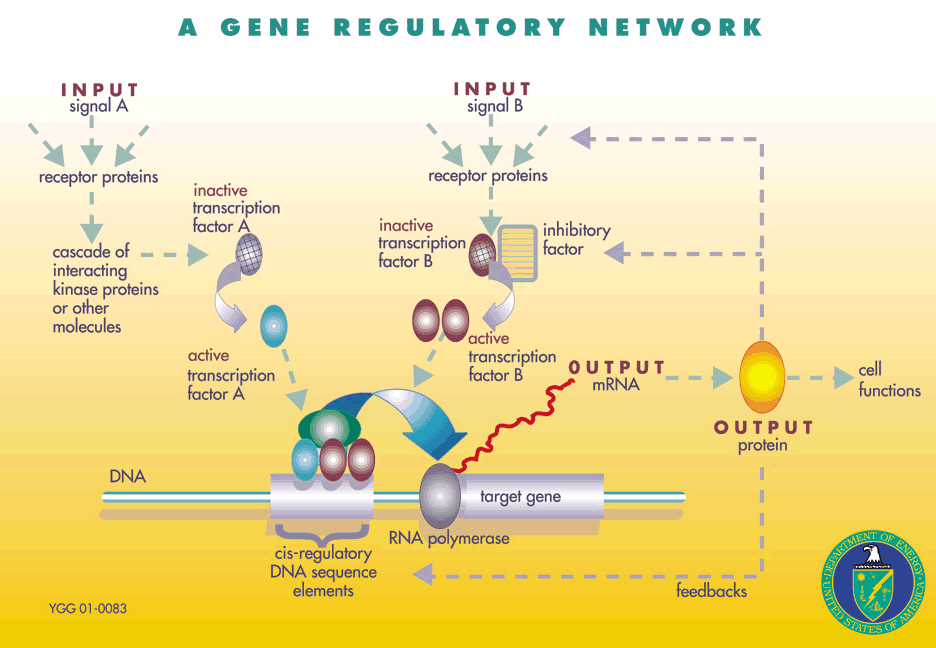
\includegraphics[width=\textwidth]{../../../gpsim/tex/diagrams/regnet2.png}
  \end{center}
}

\frame{
  \frametitle{The data}

  \begin{itemize}
  \item High-throughput measurements of nucleic acids (esp. mRNA)
  \item Detecting proteins require more targeted techniques
  \end{itemize}

  \begin{figure}[h]
    \centering
    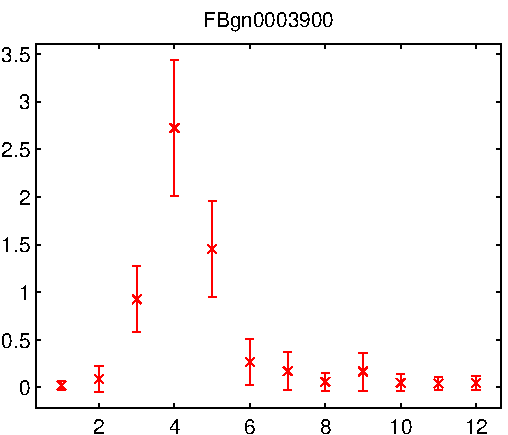
\includegraphics[width=.4\textwidth]{../../../gpsim/tex/diagrams/FBgn0003900_expression}
    \caption{Sample expression time series}
  \end{figure}
}

% \frame{
%   \frametitle{From DNA to living organisms}

%   \begin{minipage}[c]{0.5\linewidth}
%     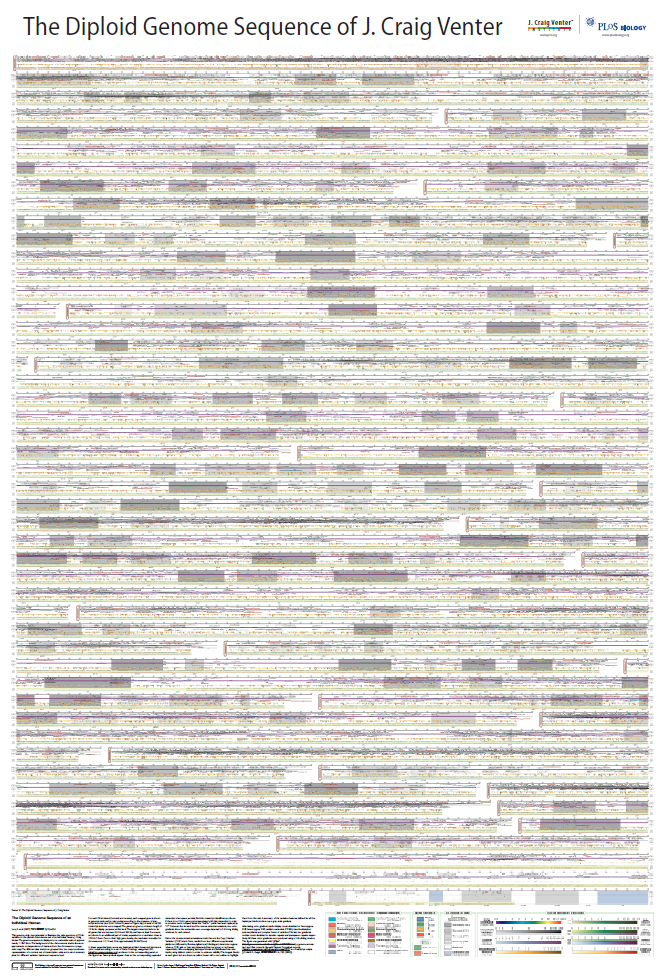
\includegraphics[width=\textwidth]{../../../gpsim/tex/diagrams/craig_venter_genome.png}
%   \end{minipage}
%   \begin{minipage}[c]{0.1\linewidth}
%     \begin{center}
%       ? \\
%       $\Rightarrow$
%     \end{center}
%   \end{minipage}
%   \begin{minipage}[c]{0.35\linewidth}
%     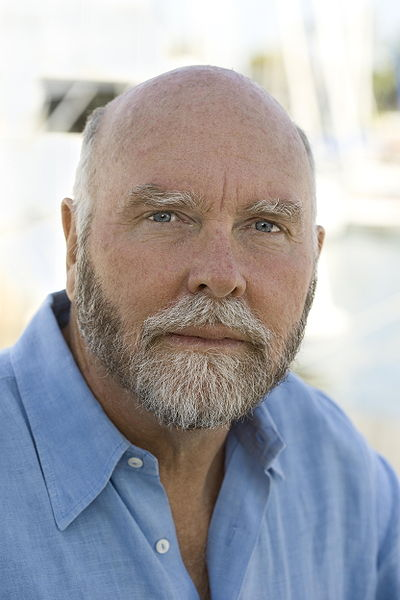
\includegraphics[width=\textwidth]{../../../gpsim/tex/diagrams/400px-Craigventer2.jpg}\\[1em]
%     {\tiny Images from PLoS Biology,\\ \url{doi:10.1371/journal.pbio.0050254}, \url{doi:10.1371/journal.pbio.0050266}}
%   \end{minipage}
% }

% \frame{
%   \frametitle{Genes and regulation}

%   \begin{itemize}
%   \item Genes known to encode proteins that perform many tasks, but%
%     \begin{itemize}
%     \item Gene expression is temporally and spatially localised
%     \item Only 1.5 \% of human DNA encodes genes
%     \end{itemize}

%   \item Numerous mechanisms of gene regulation, still poorly understood
%     \begin{itemize}
%     \item<1-> Modification of DNA (Epigenetics)
%     \item<1-| alert@2> Transcription regulation
%     \item<1-> Post-transcriptional modification
%     \item<1-> RNA transport regulation
%     \item<1-> Translation regulation
%     \item<1-> Regulation of mRNA degradation
%     \item<1-> Post-translational modifications
%     \end{itemize}
%   \end{itemize}
% }

% \frame{
%   \frametitle{Gene expression}

%   \begin{figure}
%     \centering
%     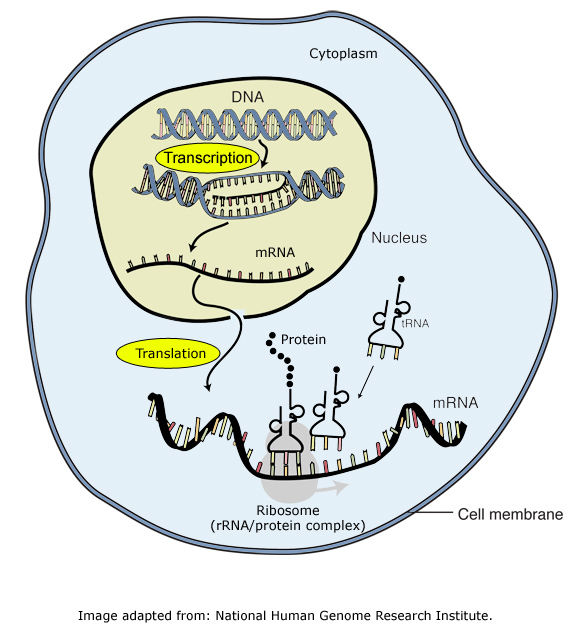
\includegraphics[width=.65\textwidth]{../../../gpsim/tex/diagrams/mrnatext_highlight_large.jpg}
%   \end{figure}
% }

% \frame{
%   \frametitle{Transcrption regulation}

%   \begin{figure}
%     \centering
%     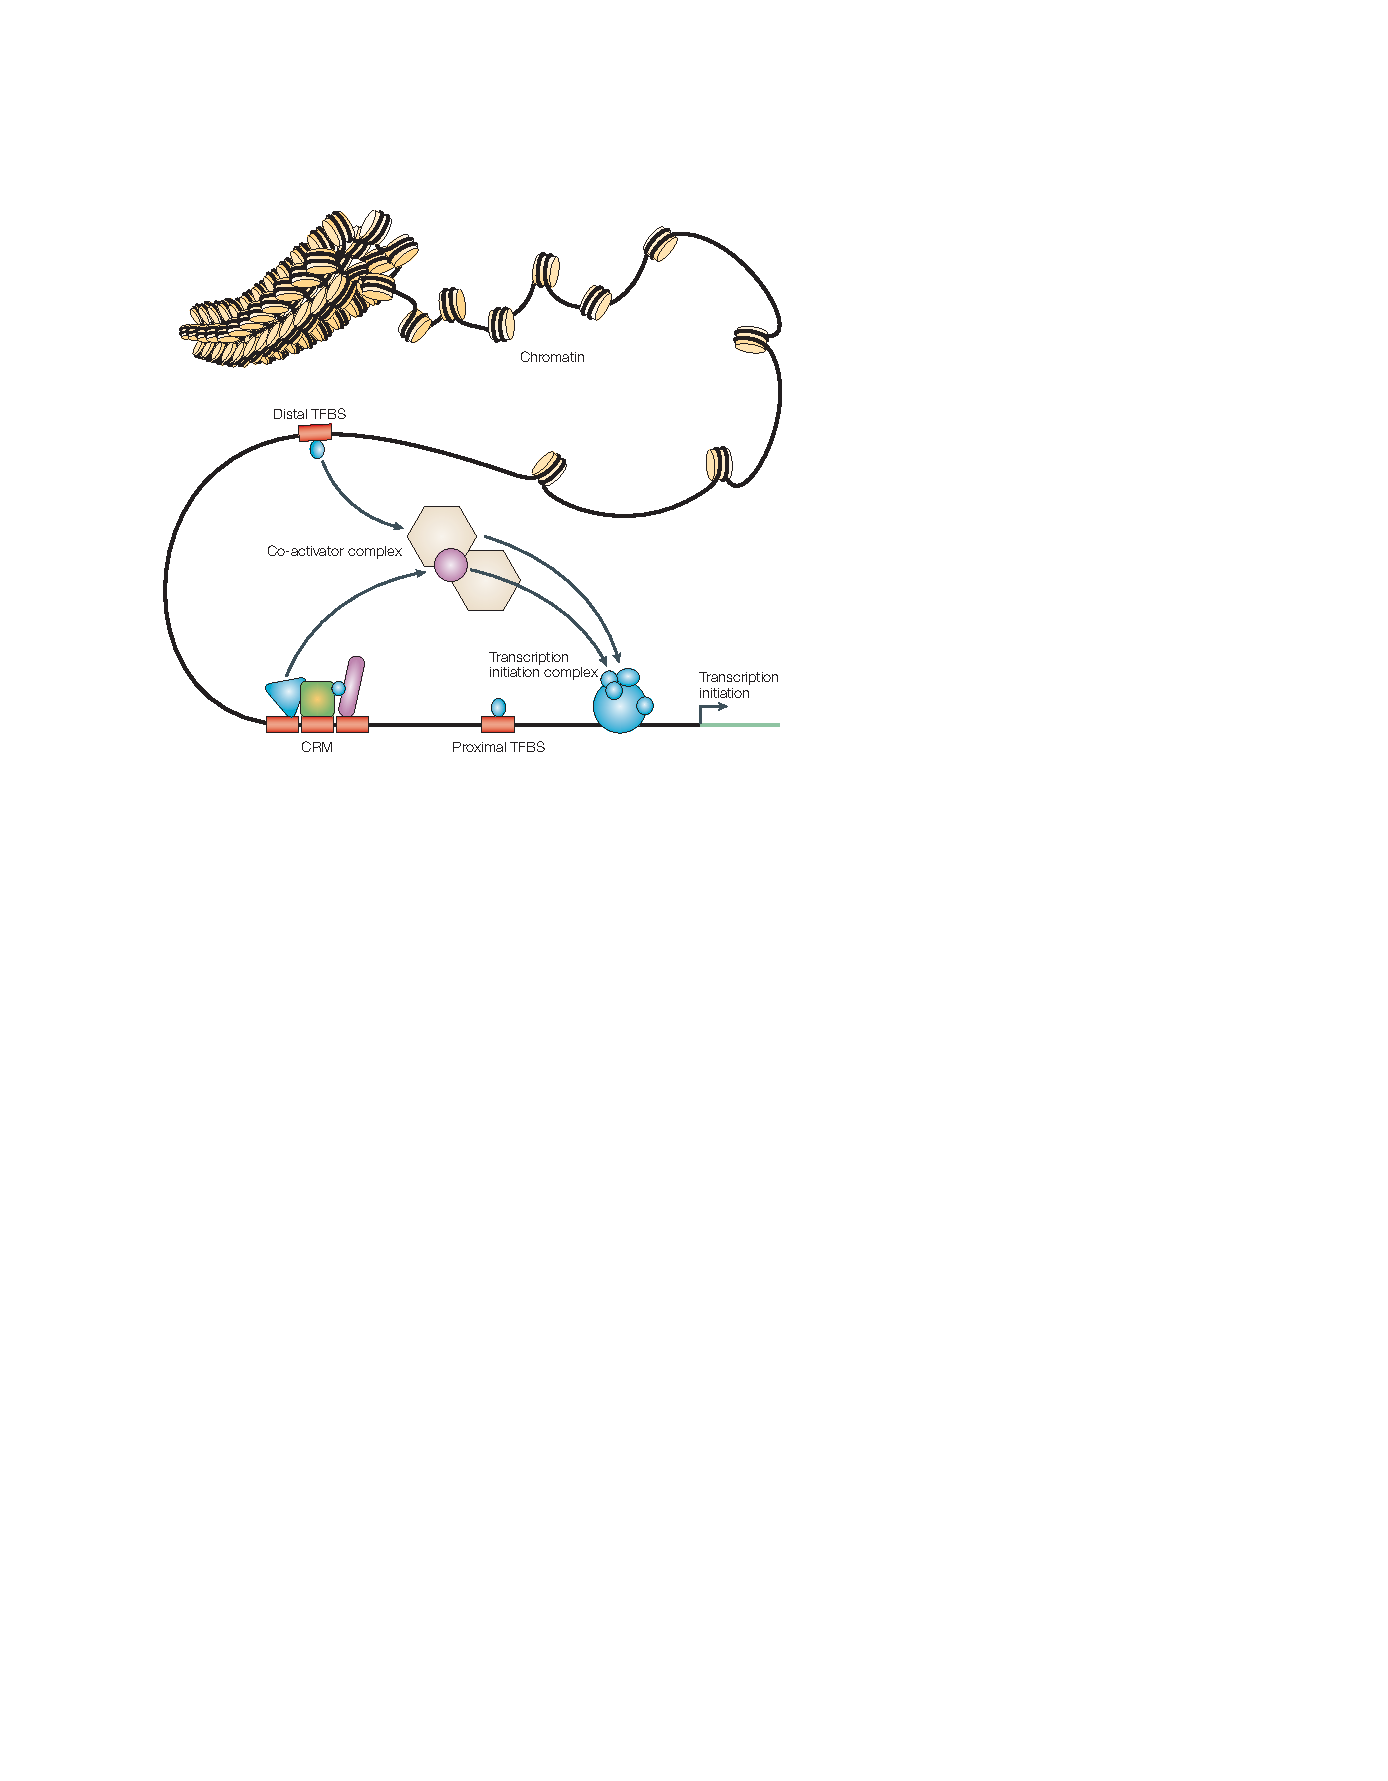
\includegraphics[width=.6\textwidth]{../../../gpsim/tex/diagrams/transcription_regulation.pdf}\\
%     {\tiny (Image from: WW Wasserman, A Sandelin. Applied bioinformatics for the identification of regulatory elements. \emph{Nat Rev Genet.} 5(4):276-87, 2004.)}
%   \end{figure}
% }

\frame{
  \frametitle{Our goal}

  \begin{itemize}
  \item To infer activities of unobserved chemical species through
    the effects they have on others
  \item Application: Infer local regulatory relationships, i.e.\
    direct targets of transcription factors (TFs)
  \item Data: time series mRNA expression data \\
    (DNA (genes) \raisebox{.4em}{$\underrightarrow{\footnotesize \text{transcription}}$}
    mRNA \raisebox{.4em}{$\underrightarrow{\footnotesize \text{translation}}$} Protein)
  \end{itemize}

%   \begin{center}
%     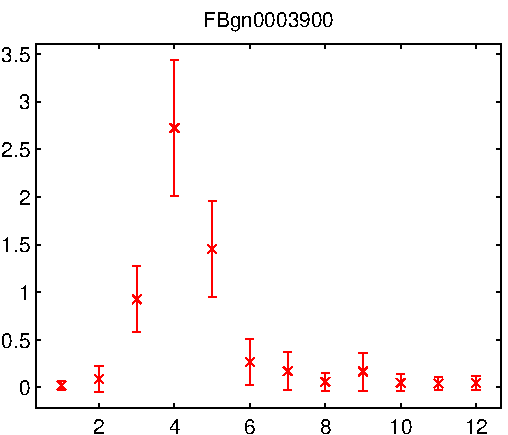
\includegraphics[width=.4\textwidth]{../../../gpsim/tex/diagrams/FBgn0003900_expression}
%   \end{center}
}


% \lyxframe{Introduction}
% \begin{itemize}
% \item Transcription factor (TF) proteins key to transcription regulation \\
% %  DNA $\rightarrow^{\text{transcription}}$ mRNA $\rightarrow^{\text{translation}}$ Protein \\
%   DNA (genes) \raisebox{.4em}{$\underrightarrow{\footnotesize \text{transcription}}$}
%   mRNA \raisebox{.4em}{$\underrightarrow{\footnotesize \text{translation}}$} Protein
% \item Measuring protein activities difficult
% \item Activities are functions of time so conventional estimation
%   methods are clearly inadequate
% \item Our approach: combine Gaussian processes and ODEs to
%   infer the activities from time series data
% \end{itemize}
% \lyxframeend{}


%\subsection{Motivation}


% \lyxframeend{}\lyxframe{Dynamical models for network modelling}

% \setbeamercovered{invisible}

% \begin{itemize}
% \item Co-regulated genes can differ greatly in their expression profiles
% \vspace{-2.5cm}

% \end{itemize}
% \begin{centercolumns}%{}

% \column{2 in}

% \begin{figure}
%  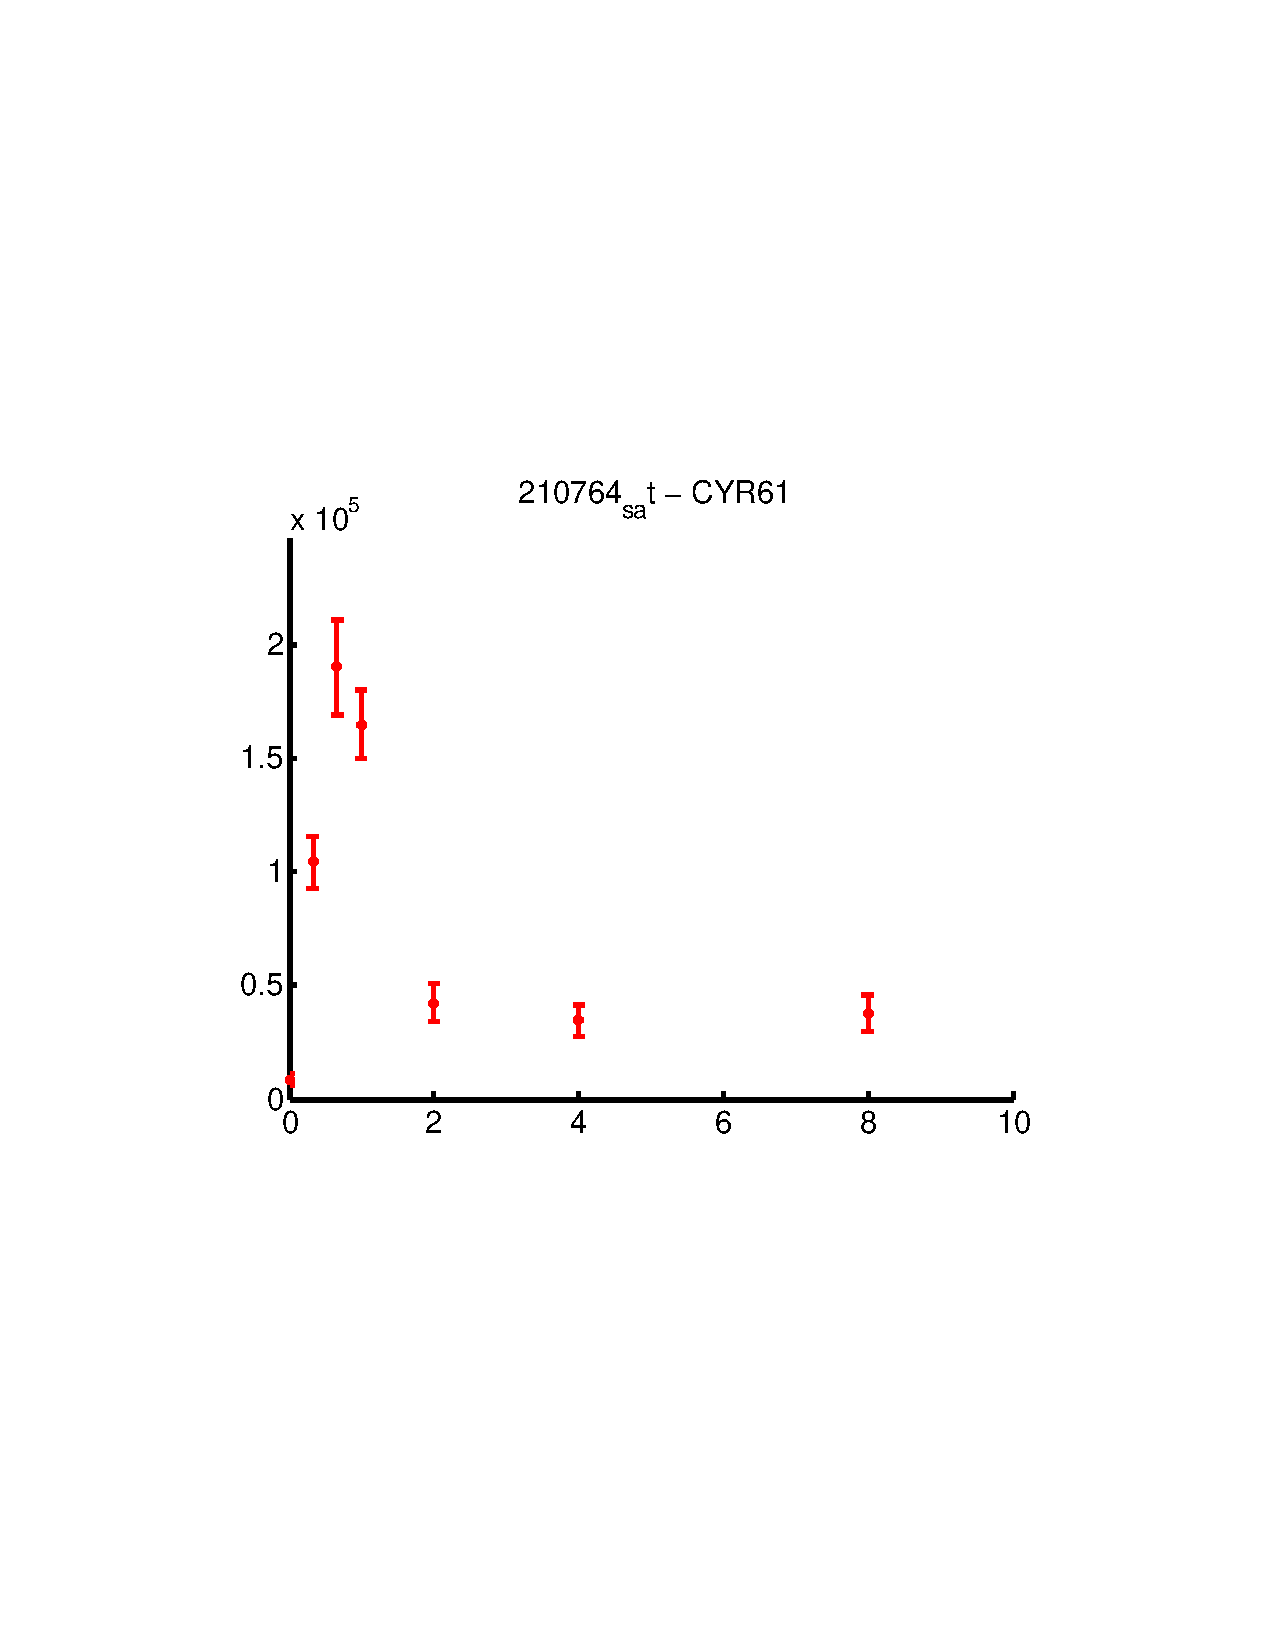
\includegraphics[clip,width=6cm]{../../../gpsim/tex/diagrams/amit_example1} 
% \end{figure}

% \column{2 in}

% \begin{figure}
%  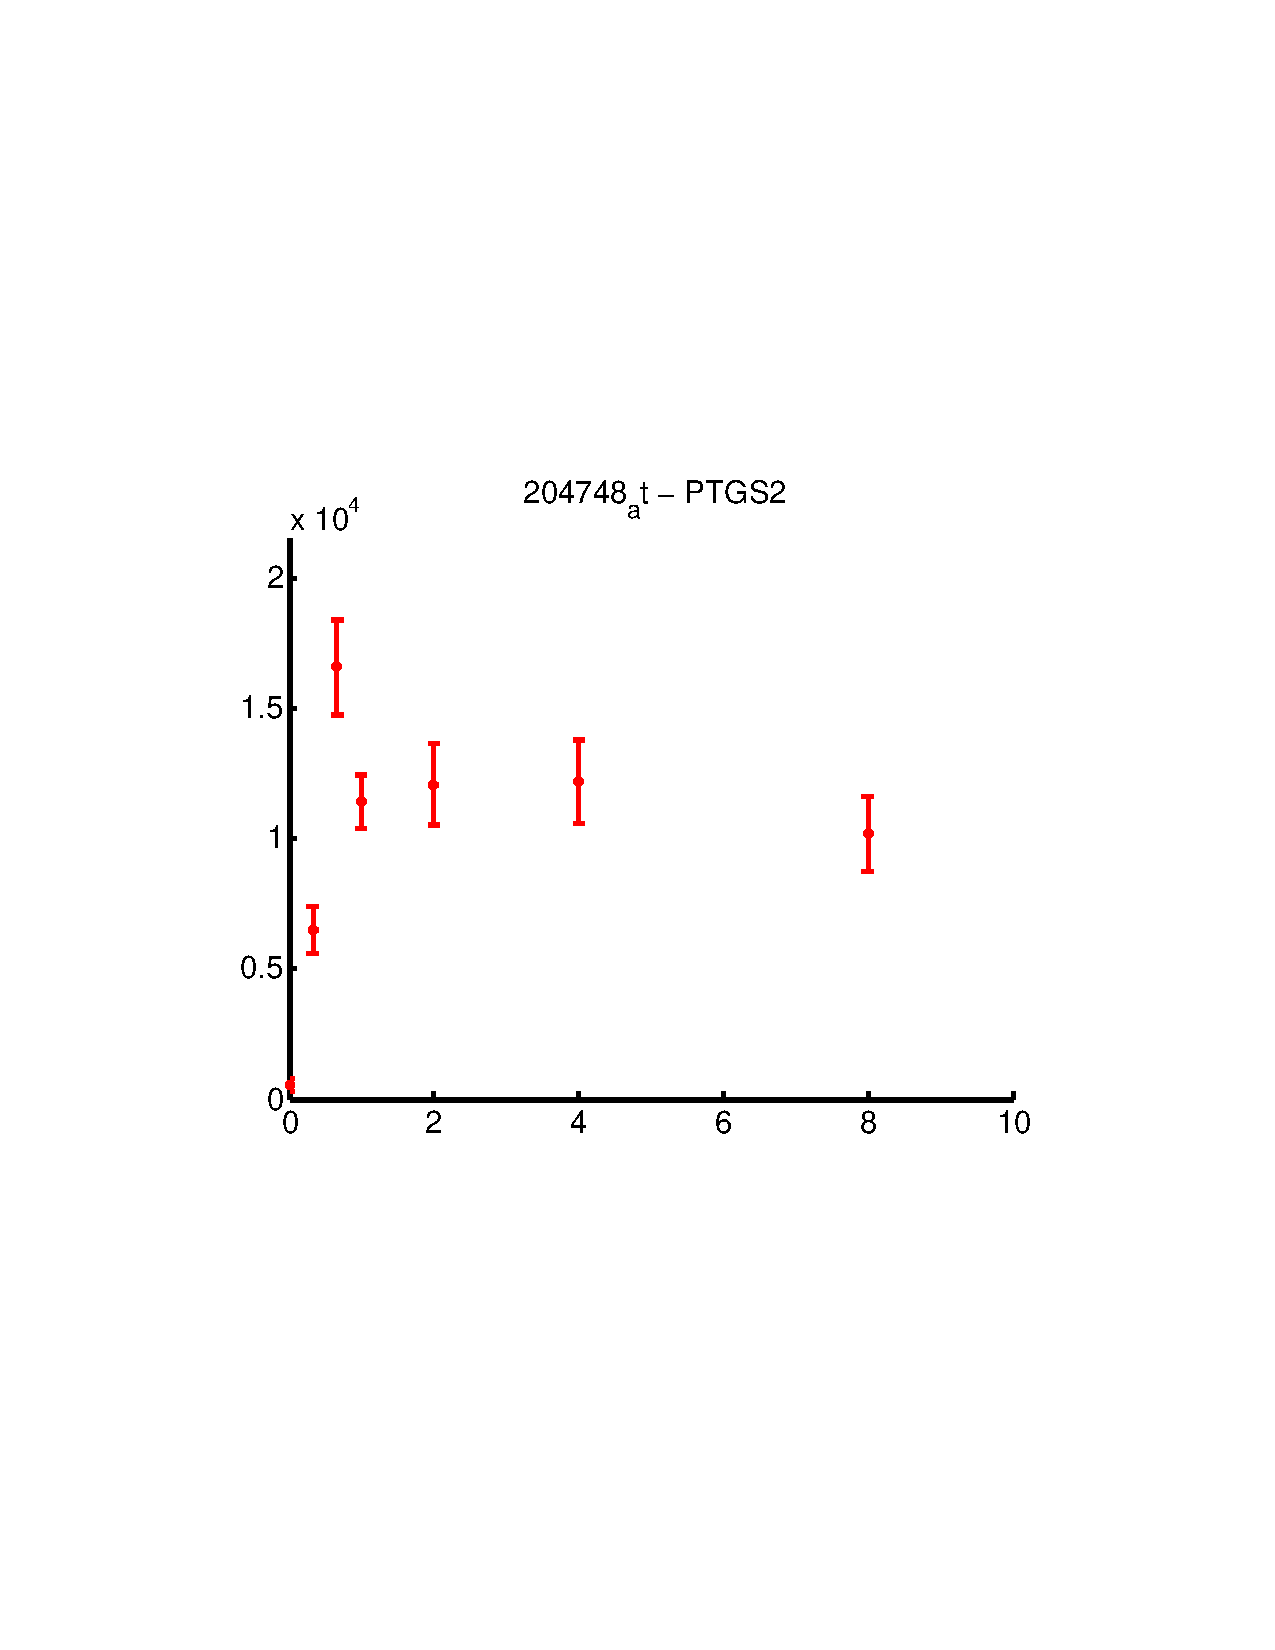
\includegraphics[clip,width=6cm]{../../../gpsim/tex/diagrams/amit_example2} 
% \end{figure}

% \end{centercolumns}%{}
% \vspace{-2cm}

% \begin{itemize}
% \item Clustering cannot be relied on to identify co-regulated genes
% \item A model-based approach is required 
% \end{itemize}


\frame{\frametitle{Outline} \tableofcontents[hideallsubsections]}

\section{ODE Models of Gene Transcription}

\frame{\frametitle{Outline} \tableofcontents[currentsection,hideallsubsections]}

\subsection{ODE Model of Activation}

\frame{
  \frametitle{The ODE model}

  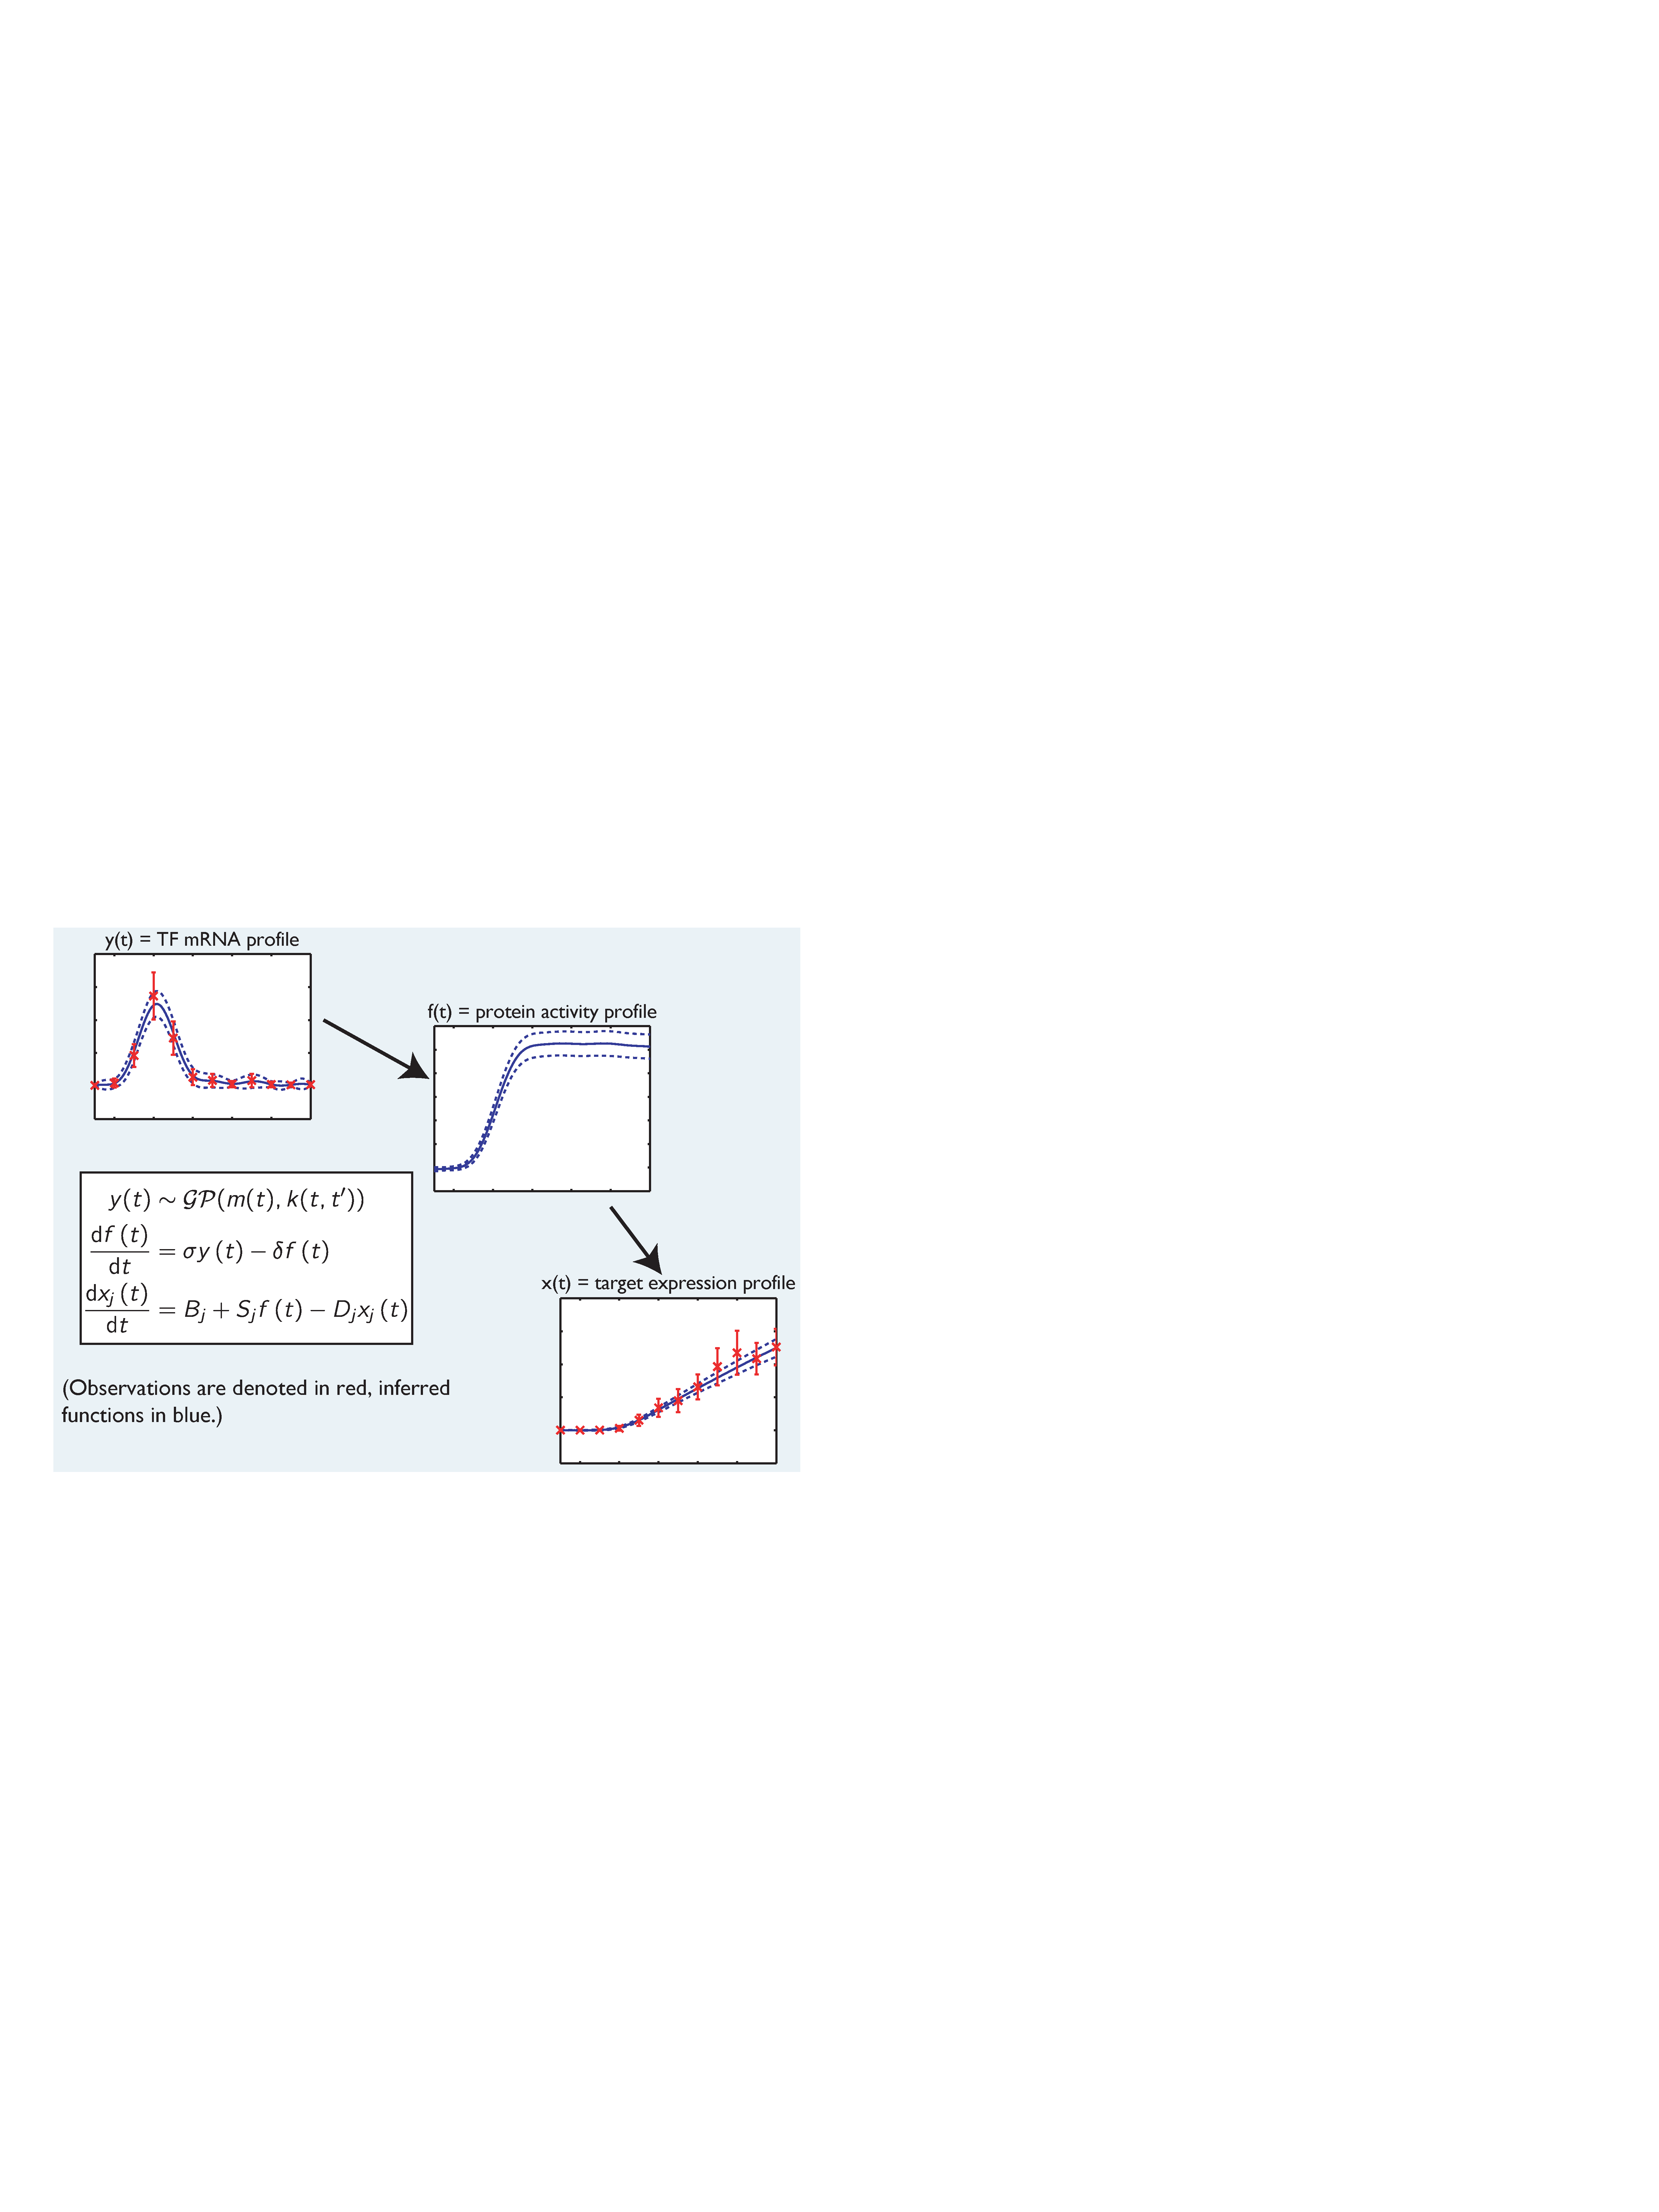
\includegraphics[width=\textwidth]{disim_model}
}

\frame{
  \frametitle{Gaussian process ODE modelling}

  \begin{itemize}
  \item Use Gaussian process priors on activity time courses
    \begin{itemize}
    \item Functional prior, specified by mean and covariance functions
    \item No need for time discretisation
    \end{itemize}
  %\item Candidate targets of the TF ranked by model likelihood
  \item Two alternatives for ``bootstrapping'' the TF protein activity
    \begin{itemize}
    \item Training set of known targets
      (cf.\ \citealp{Barenco:ranked06}, Genome Biology)
    \item Hierarchical model with TF translation from measured mRNA
    \end{itemize}
  \end{itemize}
}

\frame{
  \frametitle{Gaussian Processes}

  \begin{itemize}
  \item Gaussian Process \[
    f\left(t\right)\backsim\mathcal{GP}\left(m\left(t\right),k\left(t,t'\right)\right)\]
    where \begin{align*}
      m\left(t\right) & = \mathbb{E}\left[f\left(t\right)\right]=\left\langle f\left(t\right)\right\rangle \\
      k\left(t,t'\right) & = \mathbb{E}\left[\left(f\left(t\right)-m\left(t\right)\right)\left(f\left(t'\right)-m\left(t'\right)\right)\right]\end{align*}
  \end{itemize}
}


\frame{
  \frametitle{The joint covariance}

\textbf{RBF covariance function for $y\left(t\right)$}

\begin{center}
{\footnotesize \begin{align*}
f\left(t\right) & = \sigma\exp\left(-\delta t\right)\int_{0}^{t}y(u)\exp\left(\delta u\right)\mathrm{d}u\\
x_{i}\left(t\right) & = \frac{B_{i}}{D_{i}}+S_{i}\exp\left(-D_{i}t\right)\int_{0}^{t}f\left(u\right)\exp\left(D_{i}u\right)\mathrm{d}u.\end{align*}
}
\par\end{center}{\footnotesize \par}

\vspace{-2cm}


\begin{centercolumns}%{}


\column{4cm}

\begin{itemize}
\item Joint distribution for $x_{1}\left(t\right)$, $x_{2}\left(t\right)$,
$f\left(t\right)$ and $y\left(t\right)$.
\item Here:\vspace{0.1cm}


{\small }\begin{tabular}{|c|c|c|c|c|}
\hline 
$\delta$ & {\small $D_{1}$} & {\small $S_{1}$} & {\small $D_{2}$} & {\small $S_{2}$}\tabularnewline
\hline
\hline 
0.1 & 5 & {\small 5} & {\small 0.5} & {\small 0.5}\tabularnewline
\hline
\end{tabular}{\small \par}

\end{itemize}

\column{6cm}

\begin{center}
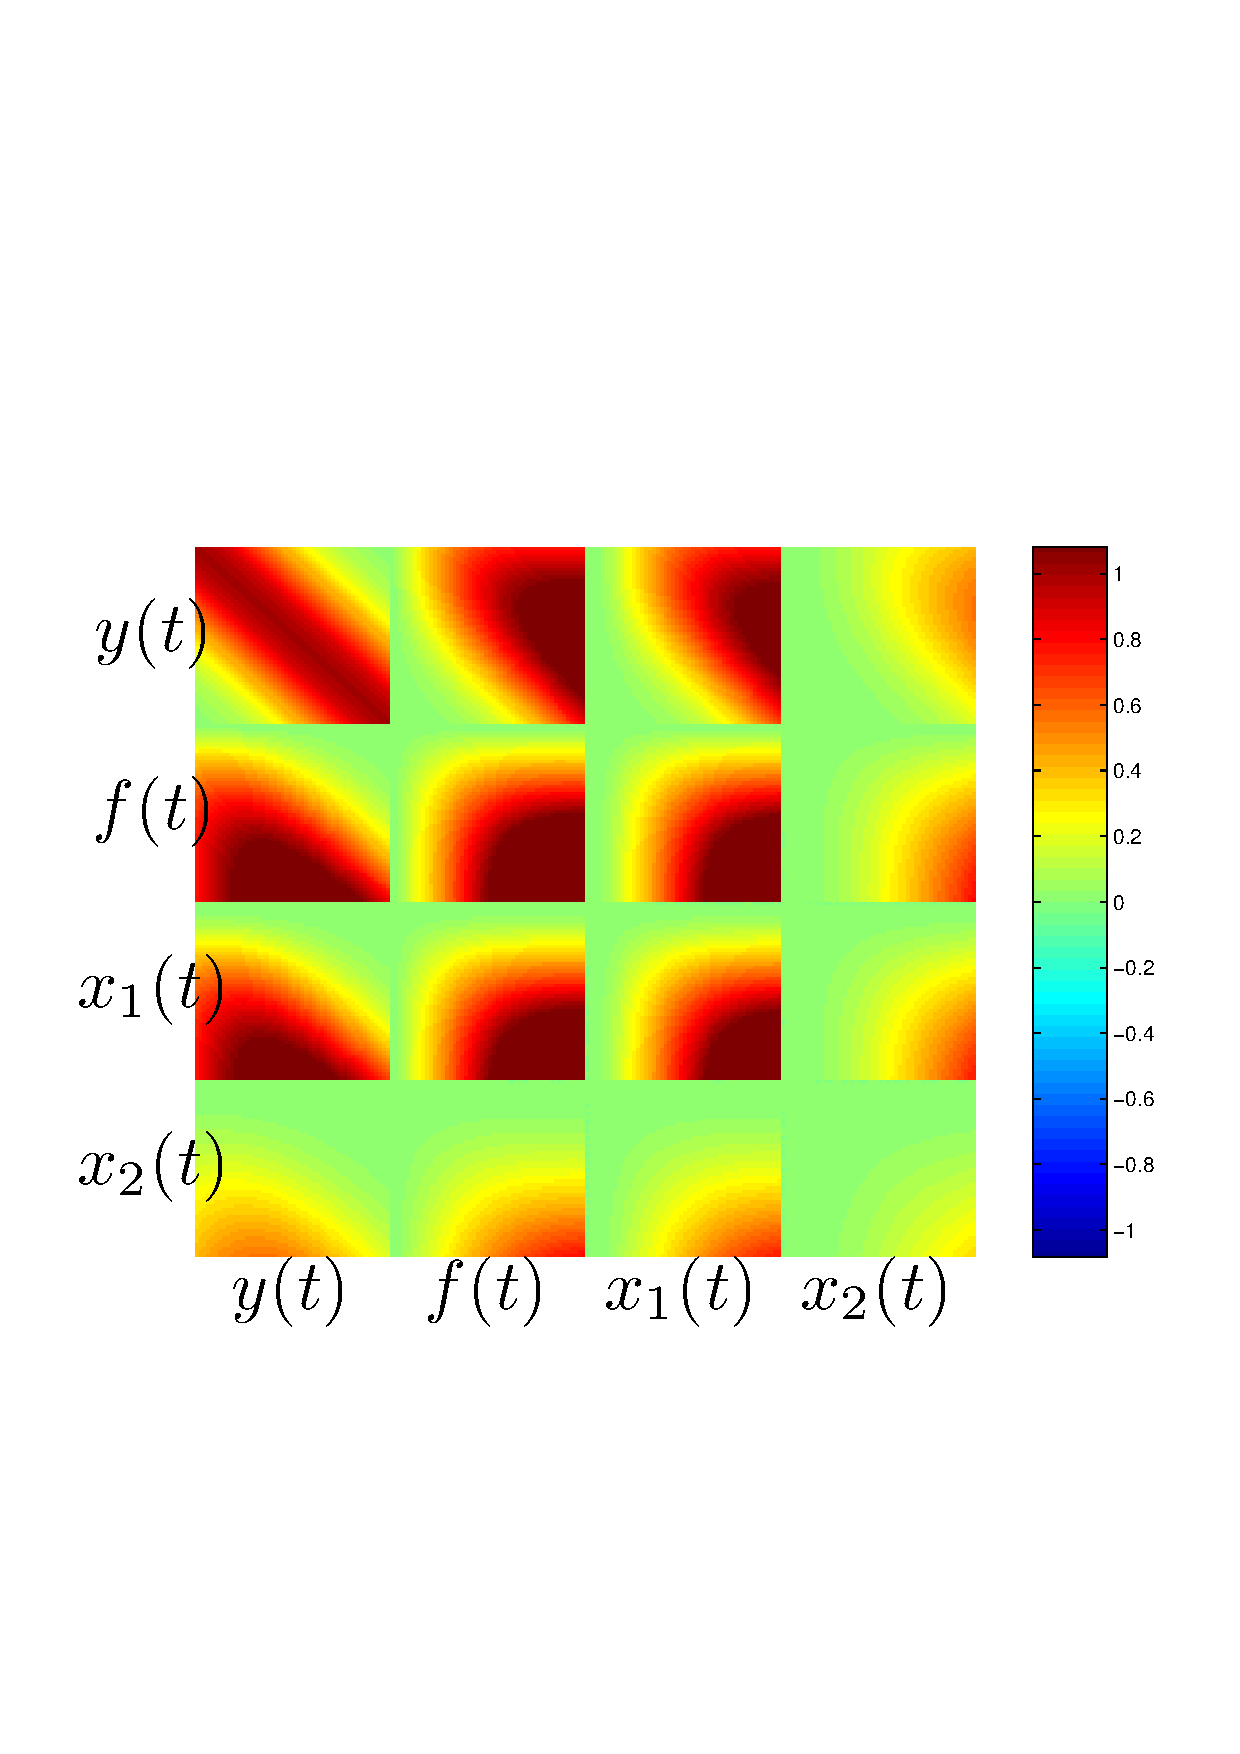
\includegraphics[width=0.8\columnwidth]{../../../gpsim/tex/diagrams/gpdisimTestKernelImage}
\par\end{center}

\end{centercolumns}%{}
}


\frame{
  \frametitle{Covariance samples}

  \begin{center}
    \includegraphics<1>[width=.8\textwidth]{../../../gpsim/tex/diagrams/disim_sample_1}
    \includegraphics<2>[width=.8\textwidth]{../../../gpsim/tex/diagrams/disim_sample_2}
  \end{center}
}


\section{Application: Transcription Factor Target Ranking}

\frame{
  \frametitle{Outline}

  \tableofcontents[currentsection,hideallsubsections]{}
}

\frame{
  \frametitle{Target ranking: motivation}

  \begin{itemize}
  \item Finding target genes of TFs is an obvious first step in
    reverse engineering gene regulatory networks
  \item Typical techniques
    \begin{itemize}
    \item Measure TF binding locations in the genome using ChIP-chip/-seq
    \item Observe gene expression in mutants with the TF disabled
      (knockouts) or overexpressed
    \end{itemize}
  \item Endless potential applications in understanding disease and
    other biological phenomena
  \end{itemize}
}

\frame{
  \frametitle{Case study: Mesoderm and muscle development in Drosophila}

  \begin{itemize}
  \item Focus on two TFs regulating mesoderm and muscle development
    in fruit fly Drosophila: Twist and Mef2
  \item Assume no post-translational regulation of these TFs
  \item Expression data: 12 time points at 1 h intervals, 3 repeats
  \item Data averaged over the whole embryo
  \end{itemize}
}

\setbeamercovered{invisible}

\frame{
  \frametitle{Application of the models to target ranking}

  \begin{itemize}
  \item First apply the two-layer model for each target gene
    independently
  \item Ranking by model likelihood
  \end{itemize}

  \setbeamercovered{invisible}
  \pause
  \begin{figure}
    \flushleft
    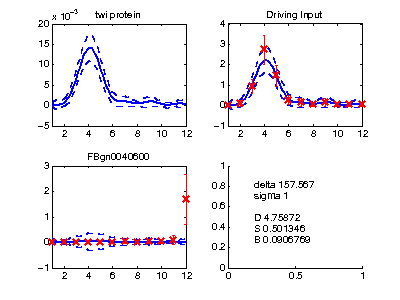
\includegraphics[width=.4\textwidth]{../../../gpsim/tex/diagrams/twi_FBgn0040600.png}
    \hspace*{-23mm}
    \includegraphics<3->[width=.4\textwidth]{../../../gpsim/tex/diagrams/twi_FBgn0000927.png}
    \hspace*{-23mm}
    \includegraphics<4->[width=.4\textwidth]{../../../gpsim/tex/diagrams/twi_FBgn0011206.png}
    \hspace*{-23mm}
    \includegraphics<5>[width=.4\textwidth]{../../../gpsim/tex/diagrams/twi_FBgn0039286.png}
    \caption{Fitted two-layer (GPDISIM) models}
  \end{figure}
}


\frame{
  \frametitle{Application of the models to target ranking}

  \begin{itemize}
  \item Need to exclude inactive genes
    \begin{itemize}
    \item Threshold the average z-score of gene activity
    \item Threshold the likelihood ratio against a model with $S=0$
    \end{itemize}
  \item Using a set of identified likely targets as a training set,
    learn multiple-target models for training set + each target
    individually
  \end{itemize}
}

\subsection{Target ranking results}

\frame{
  \frametitle{Evaluation methods}

  \begin{itemize}
  \item Evaluate the ranking methods by taking a number of top-ranked
    targets and record the number of
    ``positives''~\citep{Zinzen2009}:
    \begin{itemize}
    \item targets with ChIP-chip binding sites within 2 kb of gene
    \item (targets differentially expressed in TF knock-outs)
    \end{itemize}
  \item Compare against
    \begin{itemize}
    \item Ranking by correlation of expression profiles
    \item Ranking by $q$-value of differential expression
      in knock-outs
    \end{itemize}
  \item Optionally focus on genes with annotated expression in
    tissues of interest
  \end{itemize}
}

\frame{
  \frametitle{Results}

  \begin{center}
    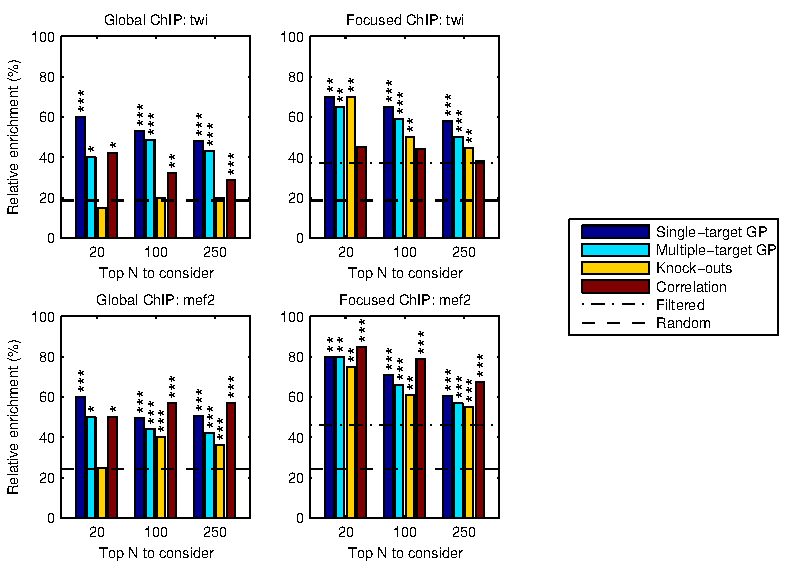
\includegraphics[width=\textwidth,trim=0mm 3mm 0mm 0mm]{../../../gpsim/tex/diagrams/dros_comparison_for_slides_2010-05-07} \\
    {\tiny '***': $p < 0.001$, '**': $p < 0.01$, '*': $p < 0.05$}
  \end{center}
}

%\frame{
%  \hspace*{-7mm}\includegraphics[width=1.18\textwidth]{PNAS-2010-Honkela-7793-8}
%}

\frame{
  \frametitle{Single-TF Target Ranking: Summary}

  \begin{itemize}
  \item The two-layer translation/transcription model provides
    impressive target ranking results
  \item Works with very short time series, even 6-7 time points
  \item More details in the paper:
  \end{itemize}
  A.~Honkela, C.~Girardot, E.~H. Gustafson, Y.-H. Liu, E.~E.~M.~Furlong, N.~D.
  Lawrence, and M.~Rattray.\\
  Model-based method for transcription factor target identification
  with limited data.\\
  {\em Proc Natl Acad Sci U S A}, 107\penalty0 (17):\penalty0
  7793--7798, Apr 2010.\\
  \url{doi:10.1073/pnas.0914285107}
}


\section{Extension: Non-linear Multiple-TF Models}

\frame{
  \frametitle{Outline}

  \tableofcontents[currentsection,hideallsubsections]{}
}

\frame{
  \frametitle{Extending the model}

  \begin{itemize}
  \item The linear single-TF model is about as far as exact inference
    takes us
  \item More complicated models require approximate techniques
    (e.g.\ MCMC)
  \item With MCMC there are no restrictions on the functional forms of
    models used
  \end{itemize}
}

\frame{
  \frametitle{The full model}

  \begin{itemize}
  \item Consider the ODE transcription regulation model for multiple
    TFs
    $$
    \frac{d x_j (t)} {d t} =
    B_j + S_j g(f_1(t),\ldots,f_I(t); \bfw_j) - D_j x_j(t)
    $$
  \item $g(\cdot )$ a positive \textcolor{blue}{sigmoidal activation function}
  \item $\bfw_j$ \textcolor{blue}{interaction weights} between the $j$th
    gene and the set of $I$ TFs
  \end{itemize}
}

\frame{
  \frametitle{Gene regulation with multiple TFs} 

$$
\frac{d x_j (t)} {d t} =
B_j + S_j g(f_1(t),\ldots,f_I(t); \bfw_j) - D_j x_j(t),
$$

\begin{itemize}
\item $g(\cdot)$ is assumed to 
     be a \textcolor{blue}{multiple-TF hill function}:
$$
g(f_1(t),\ldots,f_I(t); \bfw_j)
= \frac{\prod_{i=1}^I f_i(t)^{w_{ji}}}
{\gamma_j^{\sum_{i=1}^I w_{ji}} + \prod_{i=1}^I f_i(t)^{w_{ji}}} 
$$
where $w_{ji}$ can be both positive and negative 

\item The above can also be written as the \textcolor{blue}{sigmoid function}: 

$$
g(f_1(t),\ldots,f_I(t); \bfw_j)
= \frac{1}{1 + e^{-w_{j0}  - \sum_{i=1}^I w_{ji} \log f_i(t)}}
$$
where we defined  $w_{j0} = - \sum_{i=1}^I w_{ji} \log \gamma_j$ 
as new parameter 

\end{itemize}
}


\frame{
  \frametitle{Bayesian inference from mRNA data: priors}

$$
x_j(t) = \frac{B_j}{D_j} +  \left(A_j - \frac{B_j}{D_j}\right) e^{-D_j t} +
S_j \int_{0}^t g(f_1(u),\ldots,f_I(u); \bfw_j) e^{-D_j(t- u)} du 
$$

$$
f_i (t) = \int_0^t y_i (t) e^{- d_i (t-u)} d u
$$

\begin{itemize}

\item We place priors on: 
  \begin{itemize}
  \item \textcolor{blue}{Kinetics:} $\Theta =
    \{A_j,B_j,D_j,S_j\}_{j=1}^N$ (uniform or log normal)
  \item \textcolor{blue}{Decays} of TF mRNA: $\{d_i\}$, (uniform or
    log normal)
  \item \textcolor{blue}{Interaction} weights: $\{\bfw_j\}$, (Gaussian
    priors with optionally positivity constraints and/or spike and
    slab sparse priors)
  \item \textcolor{blue}{mRNA functions} $y_i(t)$:
    \textcolor{red}{Gaussian processes} (through a transformation that
    ensures positivity of $y_i(t)$)
  \item \textcolor{blue}{Lengthscales} of Gaussian processes (uniform
    or gamma) and \textcolor{blue}{noise variances} in the likelihoods
    (gamma)
  \end{itemize}
\end{itemize}
}



\frame{
  \frametitle{Bayesian inference from mRNA data: MCMC (Michalis)}

$$
\text{joint} 
= p(\widetilde{X}|X) p(\widetilde{Y}|Y) p(\bar{Y}_i) p(\Theta) 
 p(W) p(\{d_i\}_{i=1}^I) p(\{\sigma_j^2\}) p(\{\ell^2\}_{i=1}^I)
$$

\begin{itemize}
\item \textcolor{blue}{Many Metropolis-Hastings} steps involving
  sampling Gaussian process functions, kinetic parameters, interaction
  weights, etc.
\item We can afford training the model using MCMC in
  \textcolor{blue}{moderate-sized} networks, e.g.\ with 100 genes and
  5 TFs and 3 replicas, \textcolor{blue}{but not genome-wide} (too
  slow for that)
\item But once the model in trained, \textcolor{blue}{we can do
    genome-wide} prediction (e.g.\ gene \textcolor{blue}{target
    identification}) and this is fast
\end{itemize}
}


\frame{
  \frametitle{Experiments in Drosophila data} 

\begin{itemize}
\item Microarray dataset containing three replicas of $12$ time points
  collected hourly throughout Drosophila embryogenesis in wild-type
  embryos
\item \textcolor{blue}{$92$ target genes} 
\item \textcolor{blue}{$5$ TFs} (including 
  \textcolor{blue}{Twist and Mef2} which regulate mesoderm and muscle development)
\item ChIP information is used to define the (deterministic) sparse
  prior one interaction between TFs and target genes~\citep{Zinzen2009}
\end{itemize}
}


\frame{
  \frametitle{Experiments in Drosophila data} 

  \includegraphics<1>[width=100mm,height=70mm]{masamb/DrosTrain925TfsmRNATFs.pdf}
  \includegraphics<2>[width=100mm,height=70mm]{masamb/DrosTrain925TfsProfiles.pdf}
  \includegraphics<3>[width=100mm,height=70mm]{masamb/DrosTrain925TfsGenes1.pdf}
  \includegraphics<4>[width=100mm,height=70mm]{masamb/DrosTrain925TfsGenes2.pdf}
  \includegraphics<5>[width=100mm,height=70mm]{masamb/DrosTrain925TfsGenes3.pdf}
}

\frame{
  \frametitle{Genome-wide gene ranking/identification}

\begin{itemize}
\item The trained model 
  gives the \textcolor{blue}{posterior distribution of
    TF profiles}
\item It can be used to make (probabilistic)
  \textcolor{blue}{statements about if a
    certain TF combination regulates a test gene $*$?}
  \begin{itemize}
  \item Infer its \textcolor{blue}{interaction weights} with a suitable prior
  \item \textcolor{blue}{Compare models} restricting a set of
    interaction weights to zero
  \end{itemize}
\end{itemize}
}

\frame{
  \frametitle{Genome-wide gene ranking/identification}

  \begin{itemize}
  \item Model comparison is based on \citet{Chib95} estimate of
    marginal likelihood
  \item Fast sampling, $< 1 \text{ min}$ per gene per model
    \begin{itemize}
    \item All functions are drawn from posterior samples
    \item Relatively few parameters to sample
    \end{itemize}
  \end{itemize}
}

\frame{
  \frametitle{Multiple-TF Models: Summary}

  \begin{itemize}
  \item Realistic models of combinatorial regulation
  \item MCMC techniques applicable to genome-wide screenings
  \item Amount of available data clearly a limiting factor in
    identifying the models
  \end{itemize}
}


\section{Extension: Experimental Structure of Time Series Assays}

\frame{
  \frametitle{Outline}

  \tableofcontents[currentsection,hideallsubsections]{}
}

\frame{
  \frametitle{Molecular biology time series}

  \begin{itemize}
  \item Biological systems are dynamic, observing their time evolution
    very helpful
  \item Time series measurements of gene expression, protein activity,
    protein binding, ...
  \item Problem: most of these assays are highly disruptive to the
    sample
  \item Therefore: time series = series of independent experiments
    run for different lengths of time
  \item This has implications for modelling...
  \end{itemize}
}

\subsection{The data}

% \frame{
%   \frametitle{Outline}

%   \tableofcontents[currentsection,currentsubsection,hideothersubsections]{}
% }

\frame{
  \frametitle{Simulated molecular biology time series}

  \begin{center}
    \includegraphics<1>[width=.65\textwidth]{../../../gpsim/tex/diagrams/crosssec_example_1_1}
    \includegraphics<2>[width=.65\textwidth]{../../../gpsim/tex/diagrams/crosssec_example_2_1}
    \includegraphics<3>[width=.65\textwidth]{../../../gpsim/tex/diagrams/crosssec_example_3_1}
    \includegraphics<4>[width=.65\textwidth]{../../../gpsim/tex/diagrams/crosssec_example_4_1}
    \includegraphics<5>[width=.65\textwidth]{../../../gpsim/tex/diagrams/crosssec_example_1_2}
    \includegraphics<6>[width=.65\textwidth]{../../../gpsim/tex/diagrams/crosssec_example_2_2}
    \includegraphics<7>[width=.65\textwidth]{../../../gpsim/tex/diagrams/crosssec_example_3_2}
    \includegraphics<8>[width=.65\textwidth]{../../../gpsim/tex/diagrams/crosssec_example_4_2}
    \includegraphics<9>[width=.65\textwidth]{../../../gpsim/tex/diagrams/crosssec_example_1_3}
    \includegraphics<10>[width=.65\textwidth]{../../../gpsim/tex/diagrams/crosssec_example_2_3}
    \includegraphics<11>[width=.65\textwidth]{../../../gpsim/tex/diagrams/crosssec_example_3_3}
    \includegraphics<12>[width=.65\textwidth]{../../../gpsim/tex/diagrams/crosssec_example_4_3}
  \end{center}
}

\frame{
  \frametitle{Real gene expression time series}

  \begin{center}
    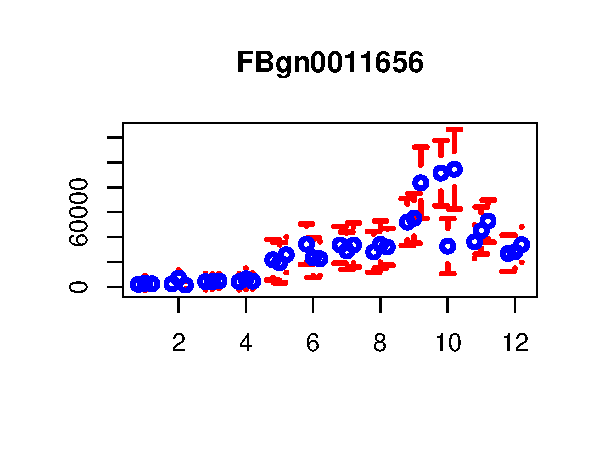
\includegraphics[width=.33\textwidth,trim=9mm 9mm 9mm 9mm]{../../../gpsim/tex/diagrams/dros_expression_series_1}
    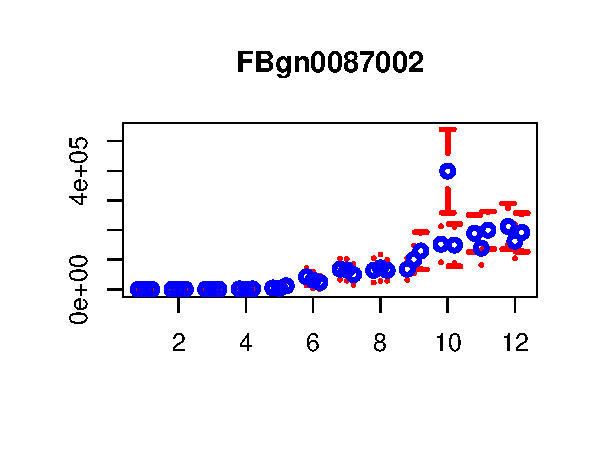
\includegraphics[width=.33\textwidth,trim=9mm 9mm 9mm 9mm]{../../../gpsim/tex/diagrams/dros_expression_series_5}
    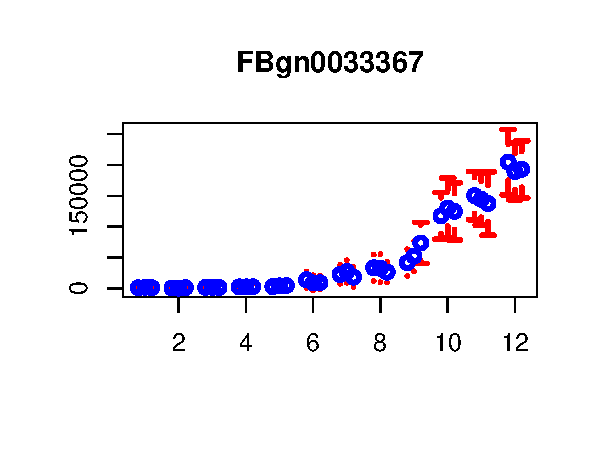
\includegraphics[width=.33\textwidth,trim=9mm 9mm 9mm 9mm]{../../../gpsim/tex/diagrams/dros_expression_series_3}\\
    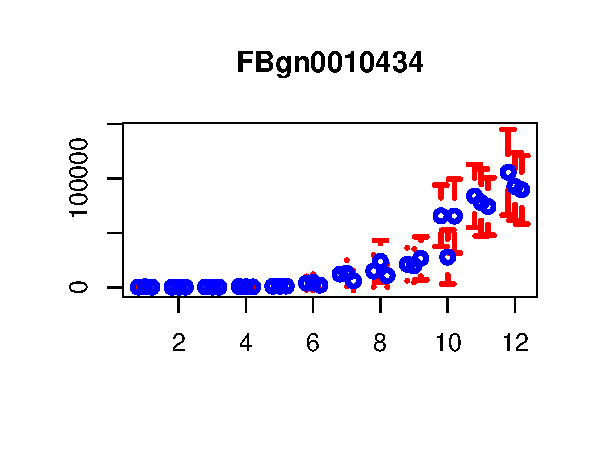
\includegraphics[width=.33\textwidth,trim=9mm 9mm 9mm 9mm]{../../../gpsim/tex/diagrams/dros_expression_series_4}
    %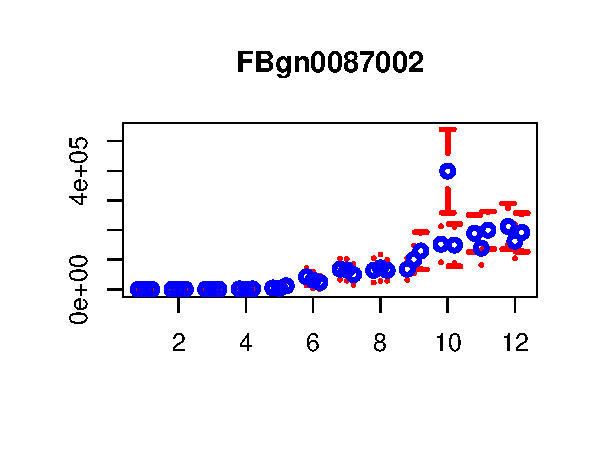
\includegraphics[width=.33\textwidth,trim=9mm 9mm 9mm 9mm]{../../../gpsim/tex/diagrams/dros_expression_series_5}
    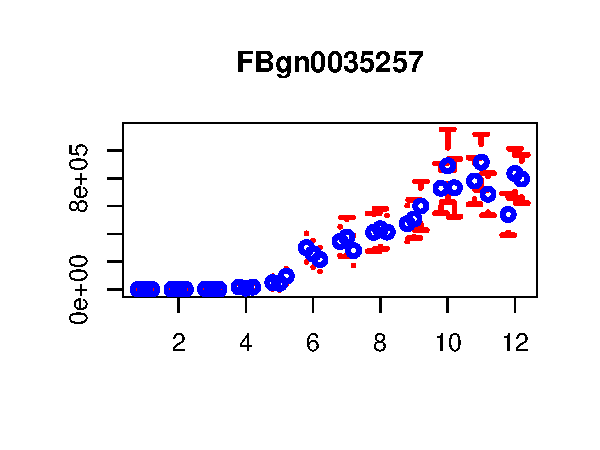
\includegraphics[width=.33\textwidth,trim=9mm 9mm 9mm 9mm]{../../../gpsim/tex/diagrams/dros_expression_series_6}
    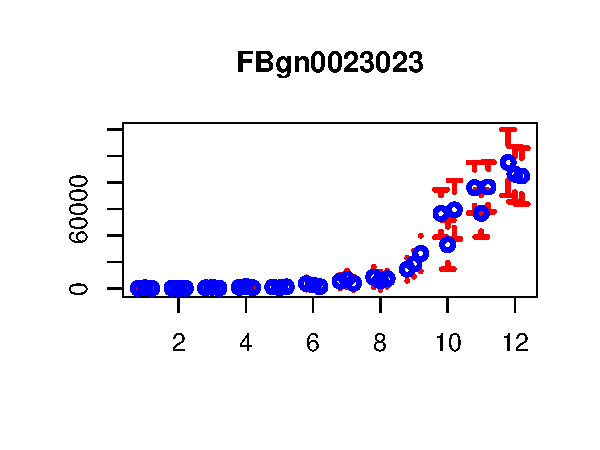
\includegraphics[width=.33\textwidth,trim=9mm 9mm 9mm 9mm]{../../../gpsim/tex/diagrams/dros_expression_series_7}\\
    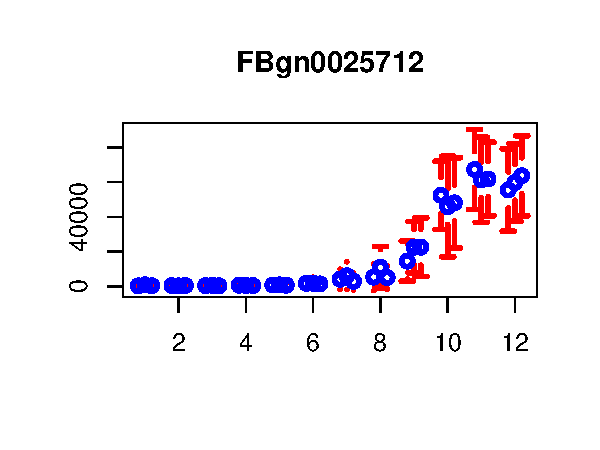
\includegraphics[width=.33\textwidth,trim=9mm 9mm 9mm 9mm]{../../../gpsim/tex/diagrams/dros_expression_series_8}
    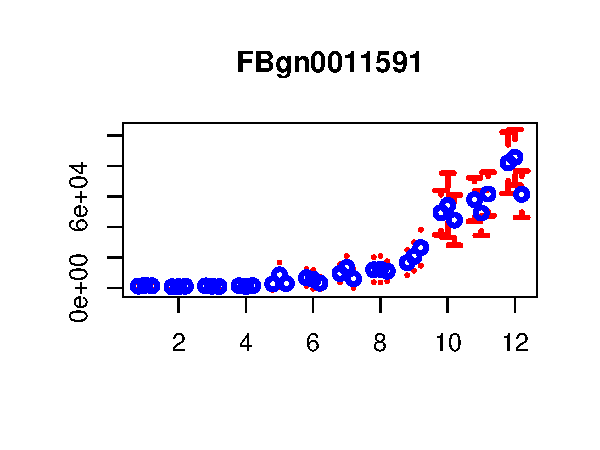
\includegraphics[width=.33\textwidth,trim=9mm 9mm 9mm 9mm]{../../../gpsim/tex/diagrams/dros_expression_series_10}
    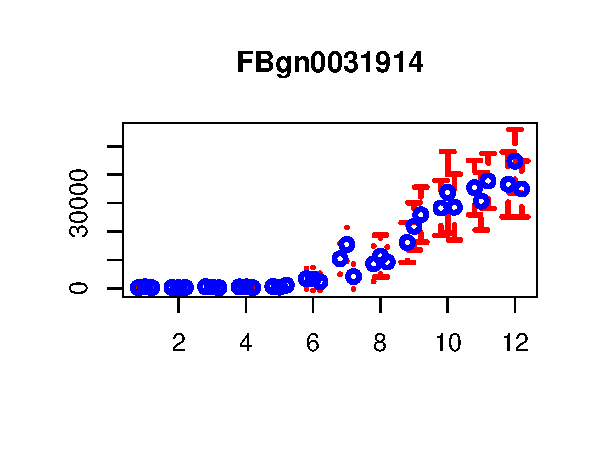
\includegraphics[width=.33\textwidth,trim=9mm 9mm 9mm 9mm]{../../../gpsim/tex/diagrams/dros_expression_series_11}
  \end{center}
}

\subsection{Models: theory}

% \frame{
%   \frametitle{Outline}

%   \tableofcontents[currentsubsection,hideothersubsections]{}
% }

\frame{
  \frametitle{Example model: Linear ODE model of transcription}

  \begin{itemize}
  \item Linear Activation Model (\citealp{Barenco:ranked06}, Genome
    Biology) \[
    \frac{\mymathrm{d}x_{j}\left(t\right)}{\mymathrm{d}t}=B_{j}+S_{j}f\left(t\right)-D_{j}x_{j}\left(t\right)\]
 
  \item $x_{j}(t)$ -- concentration of gene $j$'s mRNA 
  \item $f(t)$ -- concentration of active transcription factor 
  \item Model parameters: baseline $B_{j}$, sensitivity $S_{j}$ and
    decay $D_{j}$ 
  \item Placing a Gaussian process (GP) prior on $f(t)$ leads to
    a joint GP over all concentration profiles (\citealp{Gao:latent08},
    Bioinformatics)
  \end{itemize}
}

\frame{
  \frametitle{How to connect the model to data?}

  \begin{enumerate}
  \item Assume \myred{independent profiles} for each complete
    (biological) repeat
    \begin{itemize}
    \item Loses statistical power for extra independence assumptions
    \item Is it meaningful to order the repeats?
    \end{itemize}
  \item Assume one \myred{shared underlying profile} with independent
    observations
    \begin{itemize}
    \item Potentially sensitive to outliers
    \end{itemize}
  \end{enumerate}
}

\frame{
  \frametitle{Exchangeability analysis}

  Assume $x_j^k(t_i)$ observation of $k$th repeat of $j$th gene at $i$th time

  \begin{tabular}{lcc}
    & $x_:^k(t_i) \leftrightarrow x_:^{k'}(t_i)$ & $x_j^k(t_i) \leftrightarrow x_j^{k'}(t_i)$ \\
    & ``swap arrays'' & ``swap single gene'' \\
    \hline
    ``Reality'' & \mygreen{Yes} & \mygreen{No} \\
    1. Independent profiles & \myred{No} & \mygreen{No} \\
    2. Shared profile & \mygreen{Yes} & \myred{Yes} \\
  \end{tabular}
}

\frame{
  \frametitle{Solution: hierarchical GP model}

  \begin{itemize}
  \item Assume the underlying $f(t)$ is composed of a shared and an
    experiment-specific part $f_{ik}(t)$
\[
    \frac{\mymathrm{d}x_{j}\left(t\right)}{\mymathrm{d}t}=B_{j}+S_{j}[f_{\text{shared}}\left(t\right) + f_{ik}\left(t\right)]-D_{j}x_{j}\left(t\right)
    \]
  \item Covariance is of the same form as usual
  \item Introduces additional covariance terms for measurements from
    the same experiment
  \item Alternative parametrisations of variance of $f_{ik}(t)$
    \begin{itemize}
    \item Shared across all experiments
    \item Sampled independently for each experiment
    \end{itemize}
  \end{itemize}
}

\frame{
  \frametitle{Exchangeability analysis revisited}

  Assume $x_j^k(t_i)$ observation of $k$th repeat of $j$th gene at $i$th time

  \begin{tabular}{lcc}
    & $x_:^k(t_i) \leftrightarrow x_:^{k'}(t_i)$ & $x_j^k(t_i) \leftrightarrow x_j^{k'}(t_i)$ \\
    & ``swap arrays'' & ``swap single gene'' \\
    \hline
    ``Reality'' & \mygreen{Yes} & \mygreen{No} \\
    1. Independent profiles & \myred{No} & \mygreen{No} \\
    2. Shared profile & \mygreen{Yes} & \myred{Yes} \\
    3. Hierarchical model & \mygreen{Yes} & \mygreen{No} \\
  \end{tabular}
%   \begin{tabular}{lccc}
%     & Indep.\ profiles & Shared profile & Hierarchical \\
%     $x_:^k(t_i) \leftrightarrow x_:^{k'}(t_i)$ & \myred{No} & \mygreen{Yes} & \mygreen{Yes} \\
%     $x_j^k(t_i) \leftrightarrow x_j^{k'}(t_i)$ & \mygreen{No} & \myred{Yes} & \mygreen{No} \\
%   \end{tabular}
}

\subsection{Models: practice}

% \frame{
%   \frametitle{Outline}

%   \tableofcontents[currentsection,hideothersubsections]{}
% }

\frame{
  \frametitle{ODE model of translation and transcription}

  \begin{itemize}
  \item Assume TF is transcriptionally regulated with related mRNA
    $y(t)$
  \item This yields a system of ODEs \citep{Gao:latent08}
    \begin{align*}
      \frac{\mymathrm{d}f\left(t\right)}{\mymathrm{d}t} & =\sigma y\left(t\right)-\delta f\left(t\right)\\
      \frac{\mymathrm{d}x_{j}\left(t\right)}{\mymathrm{d}t} & =B_{j}+S_{j}f\left(t\right)-D_{j}x_{j}\left(t\right)
    \end{align*}
  \item The corresponding GP model can be derived analogously to the
    previous case
  \end{itemize}
}

\frame{
  \frametitle{Independent profiles}

  \begin{center}
    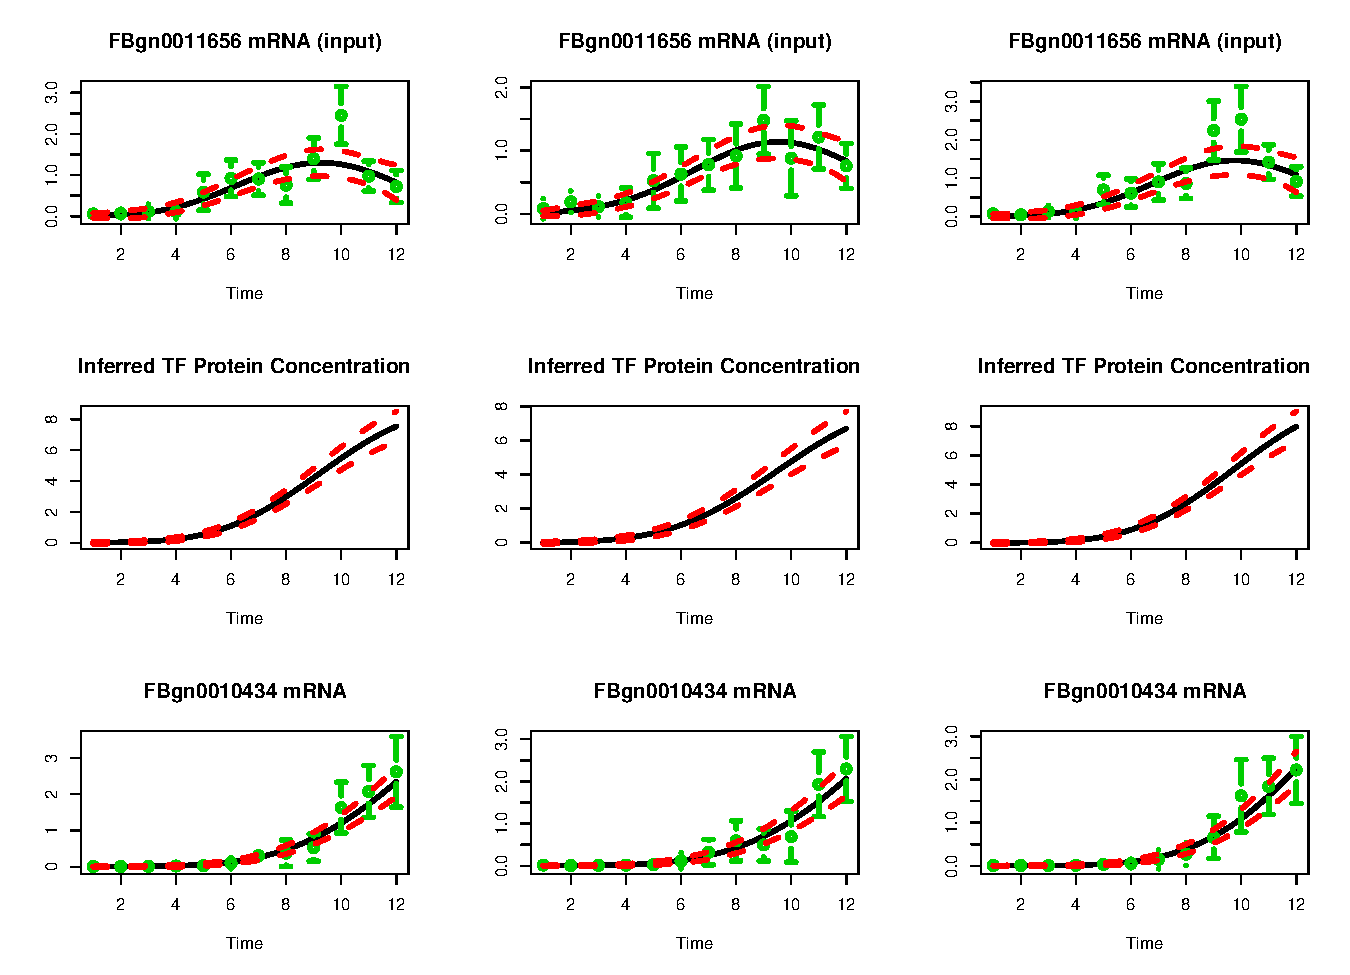
\includegraphics[scale=0.45]{../../../gpsim/tex/diagrams/old_sample_model}
  \end{center}
}

\frame{
  \frametitle{Hierarchical model}

  \begin{center}
    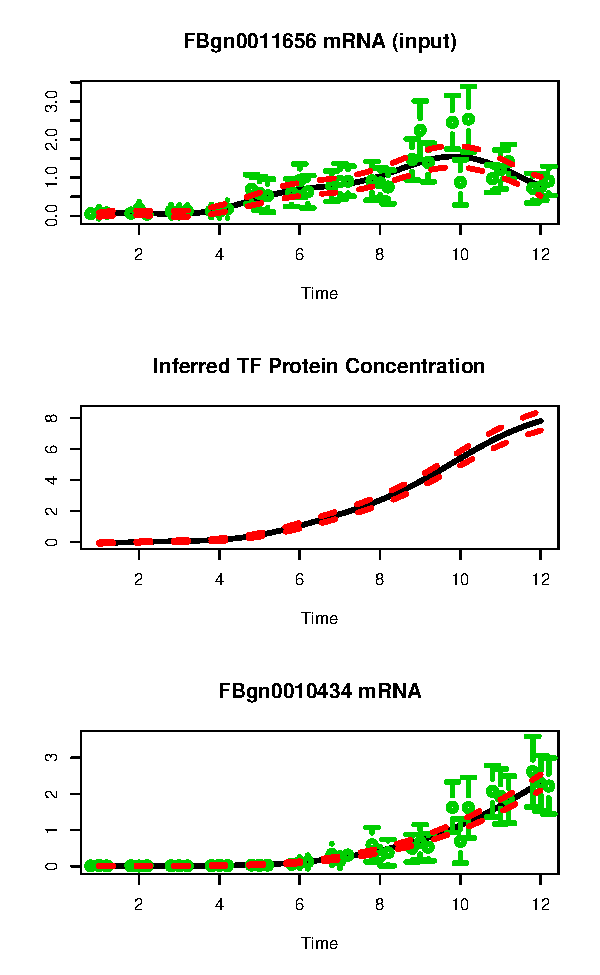
\includegraphics[scale=0.5]{../../../gpsim/tex/diagrams/hier_sample_model}
  \end{center}
}

\section{Conclusion}

% \frame{
%   \frametitle{Outline}

%   \tableofcontents[currentsection]{}
% }

\frame{
  \frametitle{Conclusion}

  \begin{itemize}
  \item Transcription factor target identification with ODE models
    \begin{itemize}
    \item Very good performance with linear single-TF models
    \end{itemize}
  \item Non-linear multiple-TF models also feasible
  \item Linear model can be extended to account for the experimental
    structure of time series assays
    \begin{itemize}
    \item Previous approaches have invalid exchangeability assumptions
    \end{itemize}
  \item Future work
    \begin{itemize}
    \item Stochastic differential equation models
    \item Incorporation of new data modalities
    \end{itemize}
  \end{itemize}
}

\frame{
  \frametitle{Acknowledgements}

  \begin{itemize}
  \item Pei Gao (University of Cambridge)
  \item Charles Girardot and Eileen Furlong  (EMBL Heidelberg)
  \end{itemize}

  \nocite{Honkela2010PNAS,Gao:latent08,GPMLBook}
}

\frame{
  \frametitle{References}

  {\tiny \bibliographystyle{pdf_abbrvnat}
    \bibliography{mpitalk}
  }{\tiny \par}
}

\frame{
  \frametitle{Now available in Bioconductor:\\ {\bf tigre} ---
    Transcription factor Inference through \\
    Gaussian process Reconstruction of Expression}

  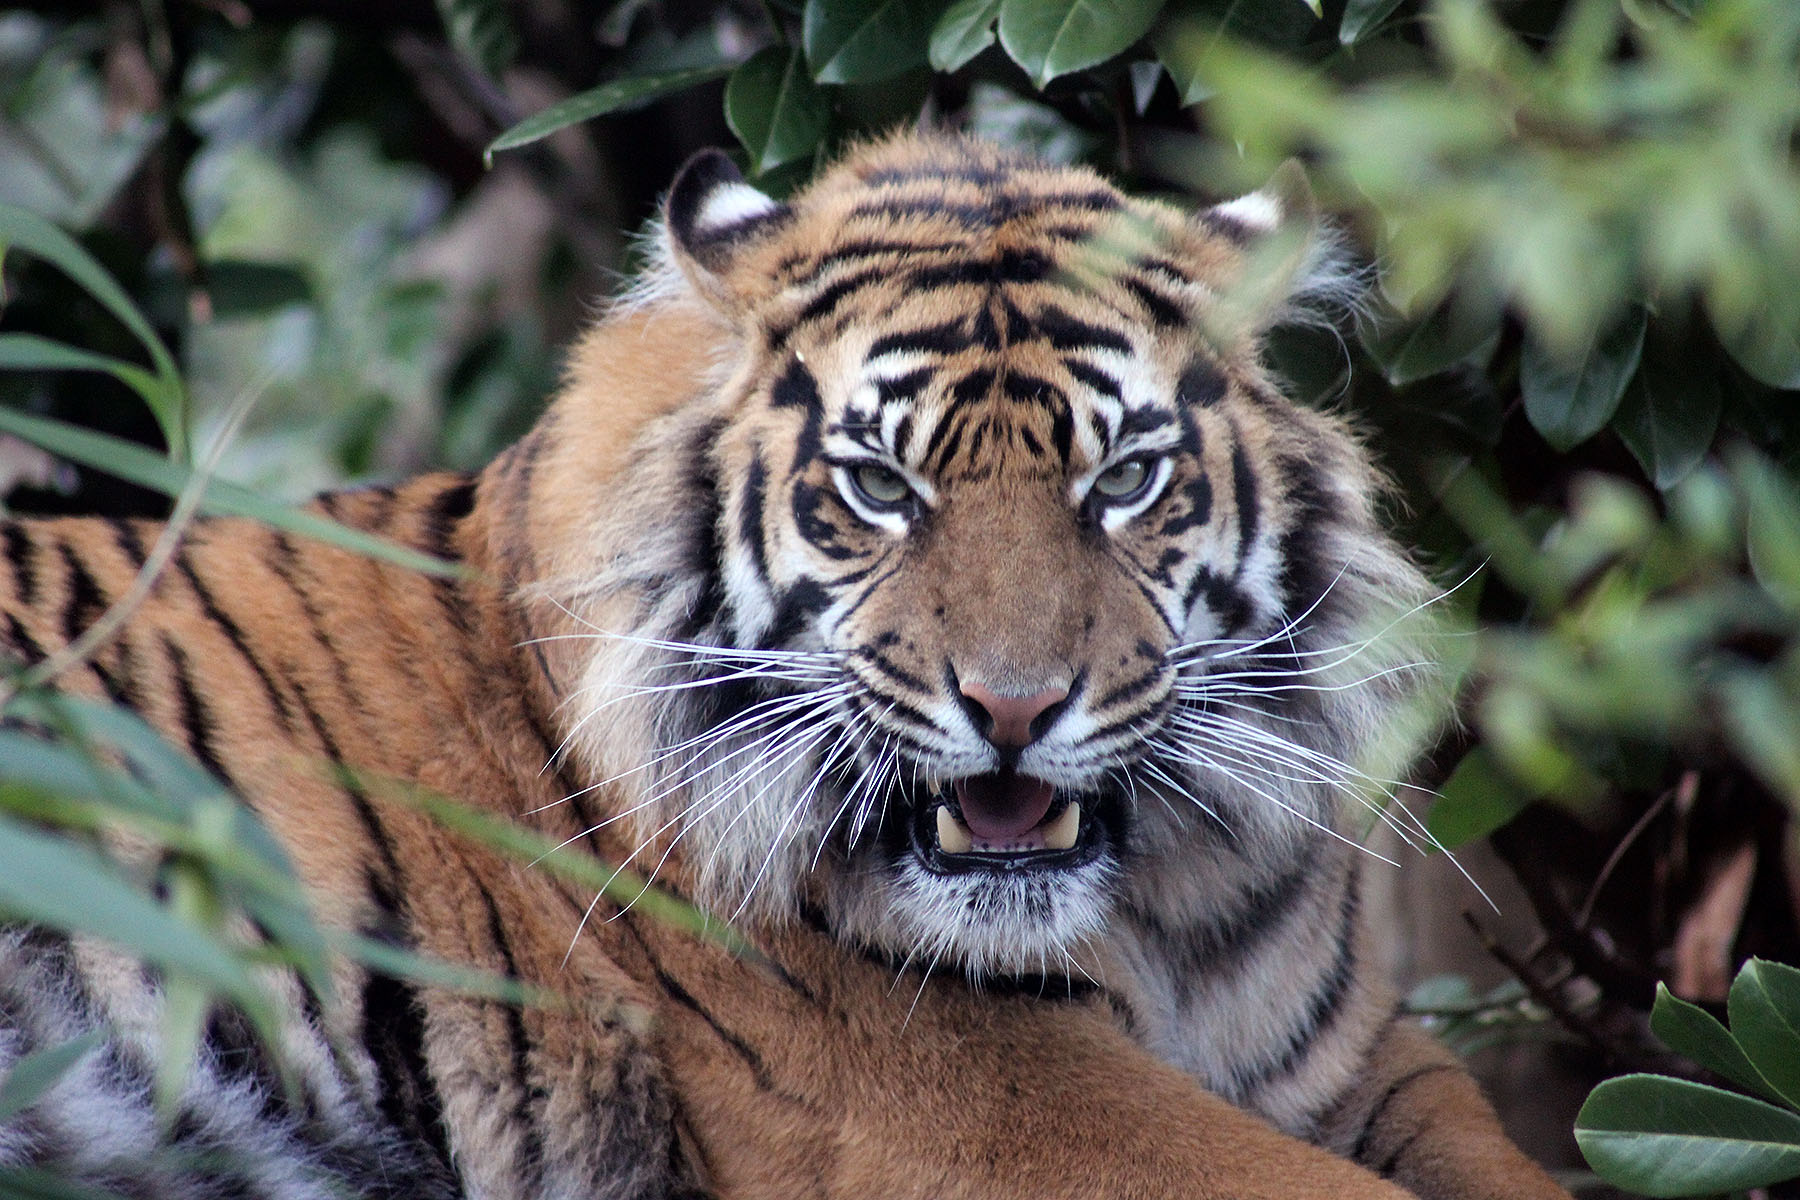
\includegraphics[width=\textwidth]{tiger_medium.jpg}
}

\end{document}
